
\documentclass[12pt]{iopart}
\pdfoutput=1
\usepackage{iopams}
\usepackage{amssymb, epsfig}
%\usepackage{amsmath, amssymb,epsfig}
\usepackage{latexsym}

%\usepackage[hypertex,hyperindex]{hyperref}
%\usepackage{showkeys}
\usepackage{graphicx}
\usepackage{color}

\newcommand{\pf}{\mbox{pf}}

\begin{document}
	
	\bibliographystyle{plain}
	\def\debproof{\noindent {\bf Proof.} }
	\def\finproof{\hfill {\small $\Box$} \\}
	%\renewcommand{\theequation}{\arabic{section}.\arabic{equation}}
	
	\makeatletter % `@' now normal "letter"
	\@addtoreset{equation}{section}
	\makeatother  % `@' is restored as "non-letter"
	\renewcommand\theequation{{\thesection}.{\arabic{equation}}}
	\title[]{}
	
	
	
	\maketitle
	\newcommand{\eps}{\varepsilon}
	\newcommand{\RR}{\mathcal{R}}
	\newtheorem{lem}{Lemma}[section]
	\newtheorem{prop}{Proposition}[section]
	\newtheorem{cor}{Corollary}[section]
	\newtheorem{thm}{Theorem}[section]
	\newtheorem{rem}{Remark}[section]
	\newtheorem{alg}{Algorithm}[section]
	\newtheorem{assum}{Assumption}[section]
	\newtheorem{definition}{Definition}[section]
	
	
	\newcounter{RomanNumber}
	\newcommand{\MyRoman}[1]{\rm\setcounter{RomanNumber}{#1}\Roman{RomanNumber}}
	
	\newcommand{\bL}{\mathbf{L}}
	\newcommand{\bH}{\mathbf{H}}
	\newcommand{\bW}{\mathbf{W}}
	\newcommand{\bP}{\mathbf{P}}
	\newcommand{\bQ}{\mathbf{Q}}
	\newcommand{\bp}{\mathbf{p}}
	\newcommand{\bq}{\mathbf{q}}
	\newcommand{\uL}{u_{_{\rm L}}}
	\newcommand{\vL}{v_{_{\rm L}}}
	\newcommand{\tuL}{\tilde u_{_{\rm L}}}
	\newcommand{\tvL}{\tilde v_{_{\rm L}}}
	\newcommand{\fL}{f_{_{\rm L}}}
	\newcommand{\gL}{g_{_{\rm L}}}
	\newcommand{\bpL}{\bp_{_{\rm L}}}
	\newcommand{\bqL}{\bq_{_{\rm L}}}
	\newcommand{\tbpL}{\tilde{\bp}_{_{\rm L}}}
	\newcommand{\tbqL}{\tilde{\bq}_{_{\rm L}}}
	\newcommand{\tbpLf}{\tilde{\bp}_{_{\rm L,1}}}
	\newcommand{\tbpLs}{\tilde{\bp}_{_{\rm L,2}}}
	\newcommand{\tbqLf}{\tilde{\bq}_{_{\rm L,1}}}
	\newcommand{\tbqLs}{\tilde{\bq}_{_{\rm L,2}}}
	\newcommand{\bn}{\nu}
	\newcommand{\bv}{\mathbf{v}}
	\newcommand{\om}{\omega}
	\newcommand{\pa}{\partial}
	\newcommand{\la}{\langle}
	\newcommand{\ra}{\rangle}
	\newcommand{\lla}{\la{\hskip -2pt}\la}
	\newcommand{\rra}{\ra{\hskip -2pt}\ra}
	\newcommand{\jj}{\|{\hskip -0.8pt} |}
	\newcommand{\al}{\alpha}
	\newcommand{\ze}{\zeta}
	\newcommand{\si}{\sigma}
	\newcommand{\ep}{\varepsilon}
	\newcommand{\na}{\nabla}
	\newcommand{\vp}{\varphi}
	\newcommand{\ga}{\gamma}
	\newcommand{\Ga}{\Gamma}
	\newcommand{\Om}{\Omega}
	\newcommand{\de}{\delta}
	\newcommand{\Th}{\Theta}
	\newcommand{\De}{\Delta}
	\newcommand{\Lam}{\Lambda}
	\newcommand{\lam}{\lambda}
	\newcommand{\tri}{\triangle}
	\newcommand{\lj}{[{\hskip -2pt} [}
	\newcommand{\rj}{]{\hskip -2pt} ]}
	\newcommand{\bks}{\backslash}
	%\newcommand{\diag}{\mathrm{diag}}
	\newcommand{\diam}{\mathrm{diam}}
	\newcommand{\osc}{\mathrm{osc}}
	\newcommand{\meas}{\mathrm{meas}}
	\newcommand{\dist}{\mathrm{dist}}
	
	\newcommand{\mL}{\mathscr{L}}
	\newcommand{\cT}{{\cal T}}
	\newcommand{\cM}{{\cal M}}
	\newcommand{\cE}{{\cal E}}
	\newcommand{\cL}{{\cal L}}
	\newcommand{\cF}{{\cal F}}
	\newcommand{\cB}{{\cal B}}
	\newcommand{\PML}{{\rm PML}}
	\newcommand{\FEM}{{\rm FEM}}
	\newcommand{\rd}{\,\mathrm{d}}
	
	\renewcommand{\i}{\mathbf{i}}
	\renewcommand{\v}{\mathbf{v}}
	\renewcommand{\u}{\mathbf{u}}
	\renewcommand{\r}{\mathbf{r}}
	\newcommand{\R}{{\mathbb{R}}}
	\newcommand{\Z}{{\mathbb{Z}}}
	\newcommand{\C}{{\mathbb{C}}}
	\renewcommand{\Re}{\mathrm{Re}\,}
	\renewcommand{\Im}{\mathrm{Im}\,}
	\renewcommand{\div}{\mathrm{div}}
	\newcommand{\curl}{\mathrm{curl}}
	\newcommand{\Curl}{\mathbf{curl}}
	
	
	%%%%%%%%%%%%%%%%%%%%%%%%%%%%%%%%%%%%%%%%%%%%%%%%%%%%%%%%%%%%%%%%%%%%
	\newcommand{\be}{\begin{eqnarray}}
	\newcommand{\ee}{\end{eqnarray}}
	\newcommand{\ben}{\begin{eqnarray*}}
		\newcommand{\een}{\end{eqnarray*}}
	\newcommand{\nn}{\nonumber}
	
	
\section{RTM phaseless: elastic; 03.15}
The RTM imaging function studied in \cite{chen2015reverse_elas} for reconstructing extended targets is
\ben
I_1(z)=-\om^2\Im\sum_{q=e_1,e_2}\int_{\Ga_s}\int_{\Ga_r}\bigg(c_pG_p(z,x_rs)q+c_sG_s(z,x_s)q\bigg)\\
\cdot\bigg(c_pG_p(z,x_r)+c_sG_s(z,x_r)\bigg)\overline{u^s_q(x_r,x_s)}ds(x_r)ds(x_s)
\een
For vector $x=(x_1,x_2)^T$, we introduce tow unit vectors $\hat{x}={x}/{|x|}:=(\hat{x}_1,\hat{x}_2)^T$ and $\tilde{x}=(-\hat{x}_2,\hat{x}_1)$. We define $A(x)=\hat{x}\hat{x}^T$ and $B(x)=\tilde{x}\tilde{x}^T$
\ben
I_2(z)=-\om^2\Im\sum_{q=e_1,e_2}\int_{\Ga_s}\int_{\Ga_r}\bigg(k_pg_p(z,x_rs)A(x_s)q+k_sg_s(z,x_s)B(x_s)q\bigg)\\
\cdot\bigg(k_pg_p(z,x_r)A(x_r)+k_sg_s(z,x_r)B(x_r)\bigg)\overline{u^s_q(x_r,x_s)}ds(x_r)ds(x_s)
\een
or
\ben
I_2(z)=-\om^2\Im\sum_{q=e_1,e_2}\int_{\Ga_s}\int_{\Ga_r}\bigg(c_pG_p(z,x_rs)q+c_sG_s(z,x_s)q\bigg)\\
\cdot\bigg(k_pg_p(z,x_r)A(x_r)+k_sg_s(z,x_r)B(x_r)\bigg)\overline{u^s_q(x_r,x_s)}ds(x_r)ds(x_s)
\een
and
\ben
I_3(z)=-\om^2\Im\sum_{q=e_1,e_2}\int_{\Ga_s}\int_{\Ga_r}\bigg(k_pg_p(z,x_rs)A(x_s)q+k_sg_s(z,x_s)B(x_s)q\bigg)\\
\cdot\bigg(k_pg_p(z,x_r)\hat{x_r}D_p(x_r,x_s)+k_sg_s(z,x_r)\tilde{x_r}D_s(x_r,x_s)\bigg)ds(x_r)ds(x_s)
\een
or
\ben
I_3(z)=-\om^2\Im\sum_{q=e_1,e_2}\int_{\Ga_s}\int_{\Ga_r}\bigg(c_pG_p(z,x_rs)q+c_sG_s(z,x_s)q\bigg)\\
\cdot\bigg(k_pg_p(z,x_r)\hat{x_r}D_p(x_r,x_s)+k_sg_s(z,x_r)\tilde{x_r}D_s(x_r,x_s)\bigg)ds(x_r)ds(x_s)
\een
where
\ben
D_p(x_r,x_s)=\frac{|\hat{x_r}^Tu_q(x_r,x_s)|^2-|\hat{x_r}^Tu^i_q(x_r,x_s))|^2}{\hat{x_r}^Tu^i_q(x_r,x_s))} \\
D_s(x_r,x_s)=\frac{|\tilde{x_r}^Tu_q(x_r,x_s)|^2-|\tilde{x_r}^Tu^i_q(x_r,x_s))|^2}{\tilde{x_r}^Tu^i_q(x_r,x_s))}
\een 
Conjecture
\ben
|I_1(z)-I_2(z)|\leq C\frac{1}{k_p R_s}, \ \ |I_2(z)-I_3(z)|\leq C\frac{1}{k_p R_s}
\een
\begin{lem}\label{kir_eq}
	We have
\ben
k_p\int_{|x|=R}g_p(z,x)A(x)\overline{G(x,y)}ds(x)=\Im G_p(z,y) +W_p(y,z)\\
k_s\int_{|x|=R}g_s(z,x)B(x)\overline{G(x,y)}ds(x)=\Im G_s(z,y) +W_s(y,z)
\een
where $|W_\alpha^{ij}(z,y)|+k_\alpha^{-1}|\nabla_z W_\alpha^{ij}(z,y)|\leq C_\alpha R^{-1}$ for some constanc $C_\alpha$ depending on $k_\alpha|z|,k_\alpha|y|$, $\alpha\in\{p,s\}$.
\end{lem}
\debproof
We first recall the following estimate for the first Hankel function in \cite[p.197]{watson1995treatise}, for any $t>0$, we have
\ben\hspace{-2cm}
H^{(1)}_0(t)=\left(\frac 2{\pi t}\right)^{1/2}e^{\i(t-\pi/4)}+R_0(t),\ \ 
H^{(1)}_1(t)=\left(\frac 2{\pi t}\right)^{1/2}e^{\i(t-3\pi/4)}+R_1(t),
\een
where $|R_j(t)|\le Ct^{-3/2}$, $j=0,1$, for some constant $C>0$ independent of $t$. By the defination of Green Tensor, we have
\ben\hspace{-2cm}
G_p(x,y)=\frac{\i}{\sqrt{8\pi}(\lambda+2\mu)}A(x-y)\frac{1}{(k_p|x-y|)^{1/2}}e^{\i k_p|x-y|-\i\frac{\pi}{4}}+O(\frac{1}{(k_p|x-y|)^{3/2}})\\ \hspace{-2cm}
G_s(x,y)=\frac{\i}{\sqrt{8\pi}\mu}B(x-y)\frac{1}{(k_s|x-y|)^{1/2}}e^{\i k_p|x-y|-\i\frac{\pi}{4}}+O(\frac{1}{(k_s|x-y|)^{3/2}})
\een
Some simple manipulation yields:
\ben 
|A(x-y)-A(x)|\leq C_1/|x|, \ \ |B(x-y)-B(x)|\leq C_2/|x| \\
 |\frac{1}{|x-y|}-\frac{1}{|x|}|\leq C_3/|x|^2 , \ \
||x-y|-(|x|-\hat{x}\cdot y)|\leq C_4/|x|
\een
where $C_i$, i=1,2,3,4 depend on $|y|$.
\ben
G_p(x,y)=\frac{\i}{\sqrt{8\pi}(\lambda+2\mu)}A(x)\frac{1}{(k_p|x|)^{1/2}}e^{\i k_p(|x|-\hat{x}\cdot y)-\i\frac{\pi}{4}}+\gamma_p(x,y)\\ 
G_s(x,y)=\frac{\i}{\sqrt{8\pi}\mu}B(x)\frac{1}{(k_s|x|)^{1/2}}e^{\i k_s(|x|-\hat{x}\cdot y)-\i\frac{\pi}{4}}+\gamma_s(x,y) \\
g_\alpha(x,y)=\frac{\i}{\sqrt{8\pi}\mu}\frac{1}{(k_\alpha|x|)^{1/2}}e^{\i k_s(|x|-\hat{x}\cdot y)-\i\frac{\pi}{4}}+\gamma(x,y)
\een
where $|\gamma_\alpha(x,y)|\leq C(k_\alpha|x|)^{-3/2}$ for some constant $C$ depending on $k_\alpha|y|$, $\alpha\in\{p,s\}$.
\finproof

Now we turn to the analysisi of the imaging function $I_3(z)$. We first observe that:
\ben
D_p(x_r,x_s)=\hat{x_r}^T\overline{u^s_q}+\frac{|\hat{x_r}^Tu^s_q(x_r,x_s)|^2}{\hat{x_r}^Tu^i_q(x_r,x_s))}+\frac{(\hat{x_r}^Tu^s_q(x_r,x_s))(\hat{x_r}^T\overline{u^i_q(x_r,x_s)})}{\hat{x_r}^Tu^i_q(x_r,x_s))}  \\ 
D_s(x_r,x_s)=\tilde{x_r}^T\overline{u^s_q}+\frac{|\tilde{x_r}^Tu^s_q(x_r,x_s)|^2}{\tilde{x_r}^Tu^i_q(x_r,x_s))}+\frac{(\tilde{x_r}^Tu^s_q(x_r,x_s))(\tilde{x_r}^T\overline{u^i_q(x_r,x_s)})}{\tilde{x_r}^Tu^i_q(x_r,x_s))}
\een
\begin{lem}
We have $|u^s_q(x_r,x_s)|\leq C(1+\|T\|)(k_p R_r)^{-1/2}(k_p R_s)^{-1/2}$ for any $x_r\in \Ga_r,x_s\in\Ga_s$, where the constant C may depend on $kd_D$ bu is independent of $k_p,k_s,d_D, R_r,R_s$.
\end{lem}
\section{Numerical Experiment}

\begin{figure}
	\centering
	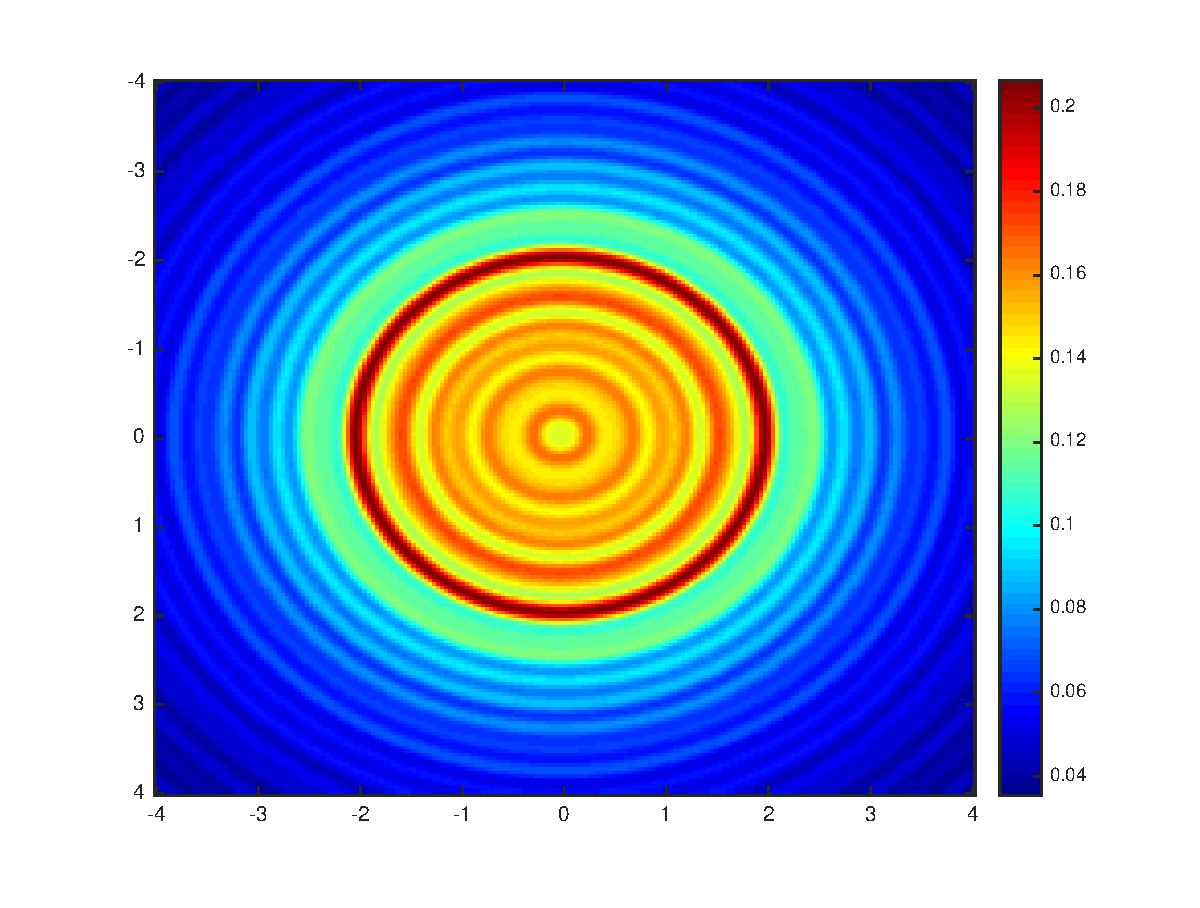
\includegraphics[width=0.24\textwidth]{./graphic_phase/circle_r_10_k_4_vector.eps}
	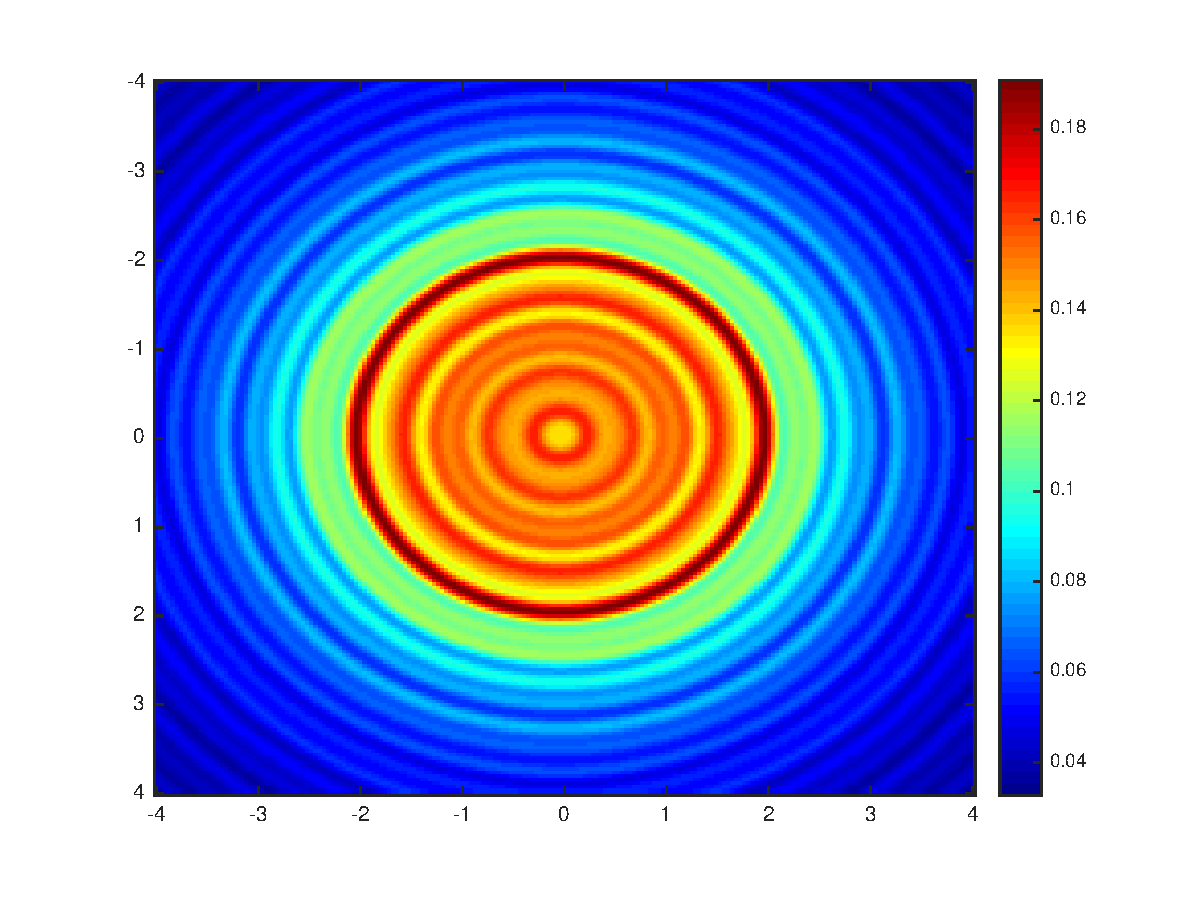
\includegraphics[width=0.24\textwidth]{./graphic_phase/circle_r_10_k_4_scalar.eps}
	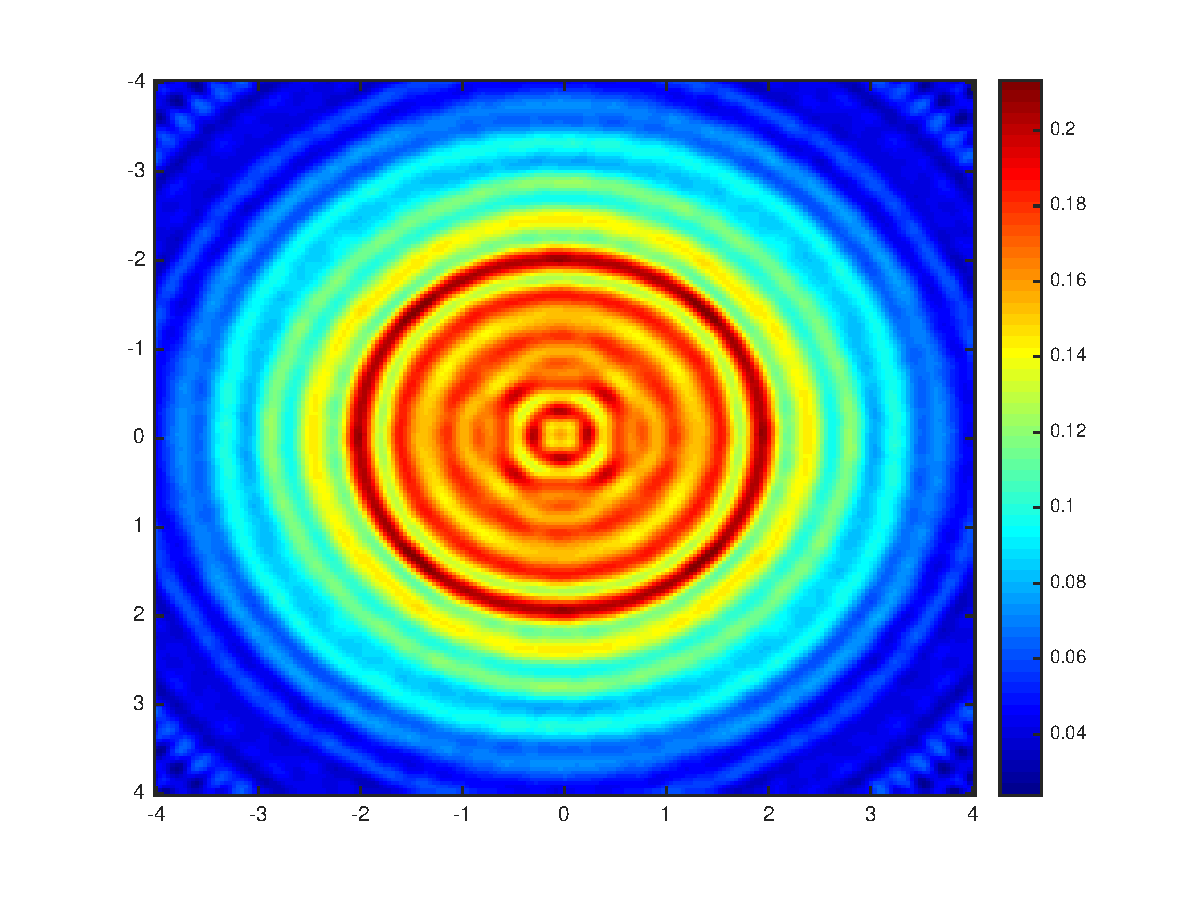
\includegraphics[width=0.24\textwidth]{./graphic_phase/circle_r_10_k_4_phaseless_n_128_bias_100.eps}
	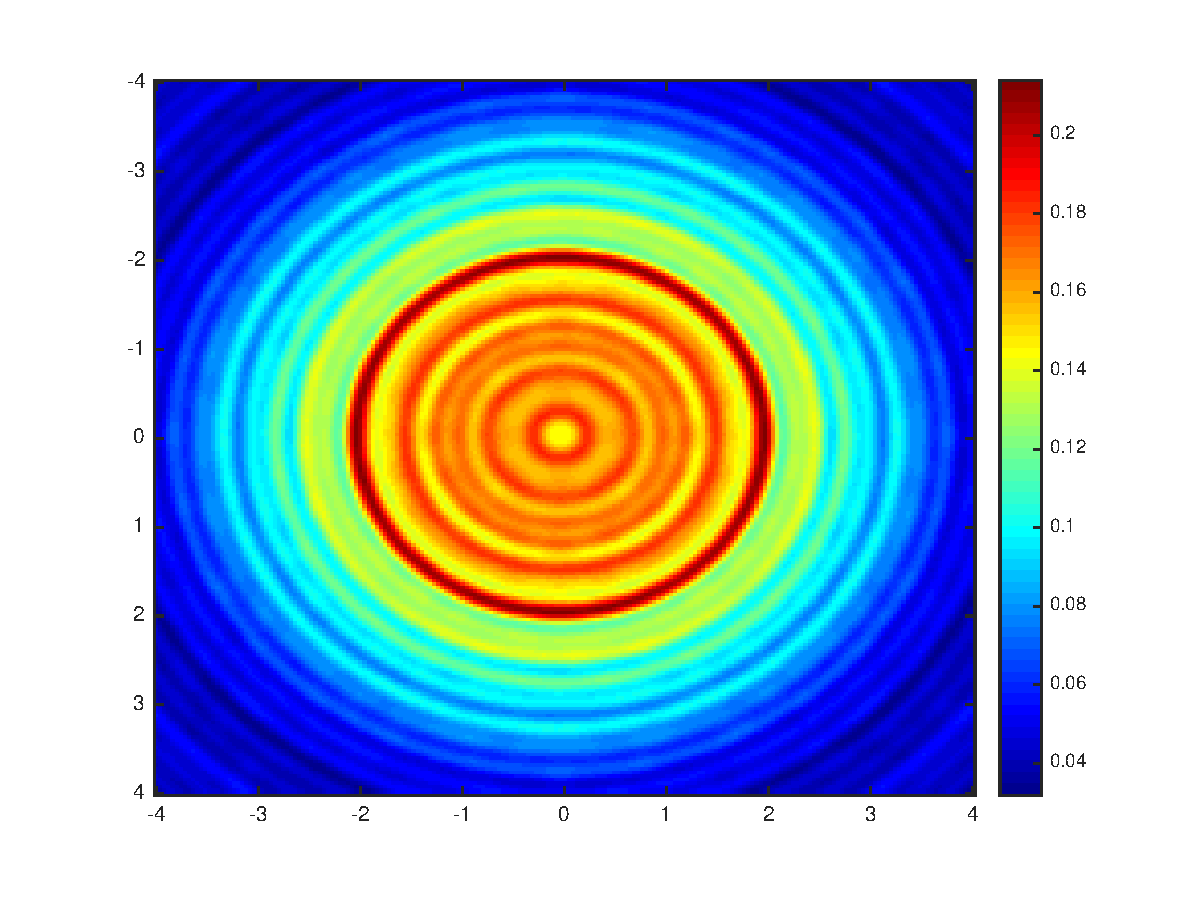
\includegraphics[width=0.24\textwidth]{./graphic_phase/circle_r_10_k_4_phaseless_n_512_bias_100.eps}
	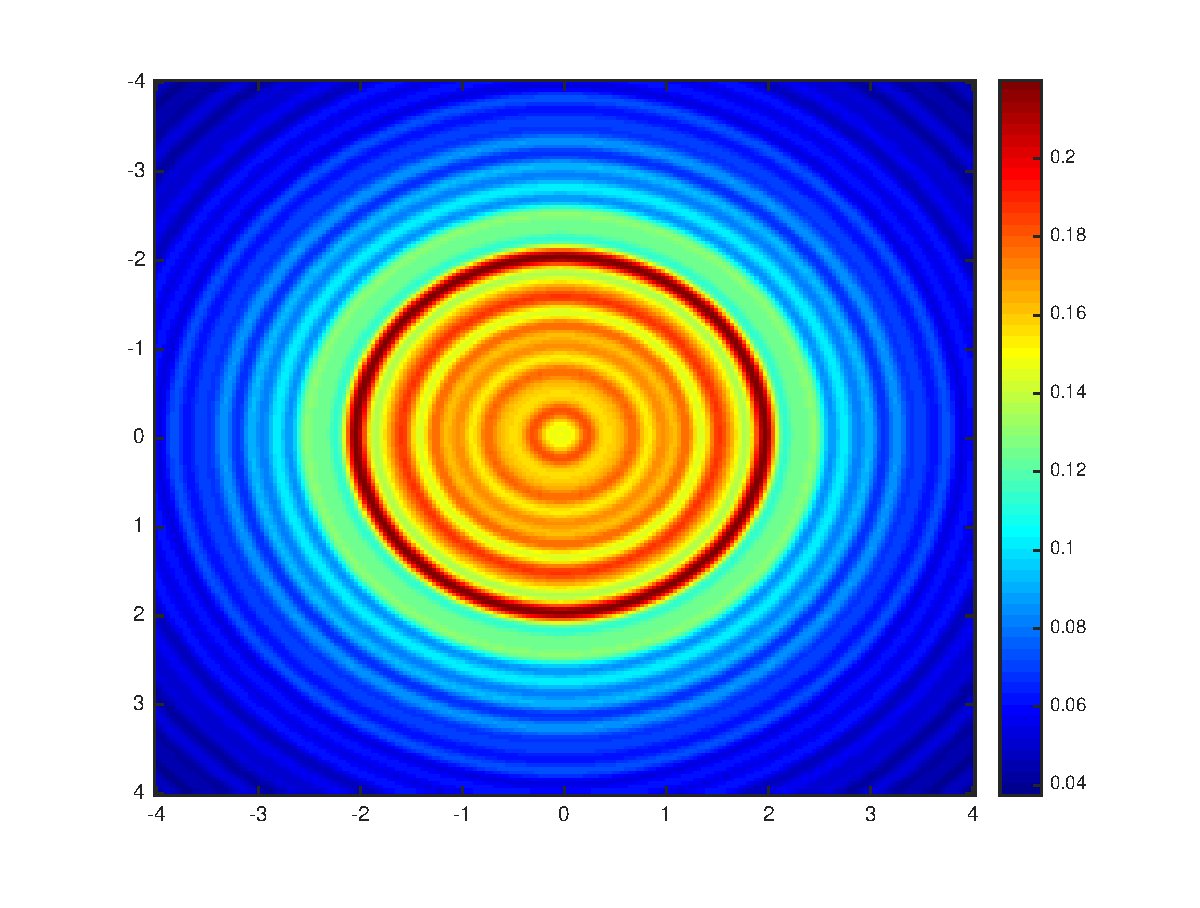
\includegraphics[width=0.24\textwidth]{./graphic_phase/circle_r_100_k_4_vector.eps}
	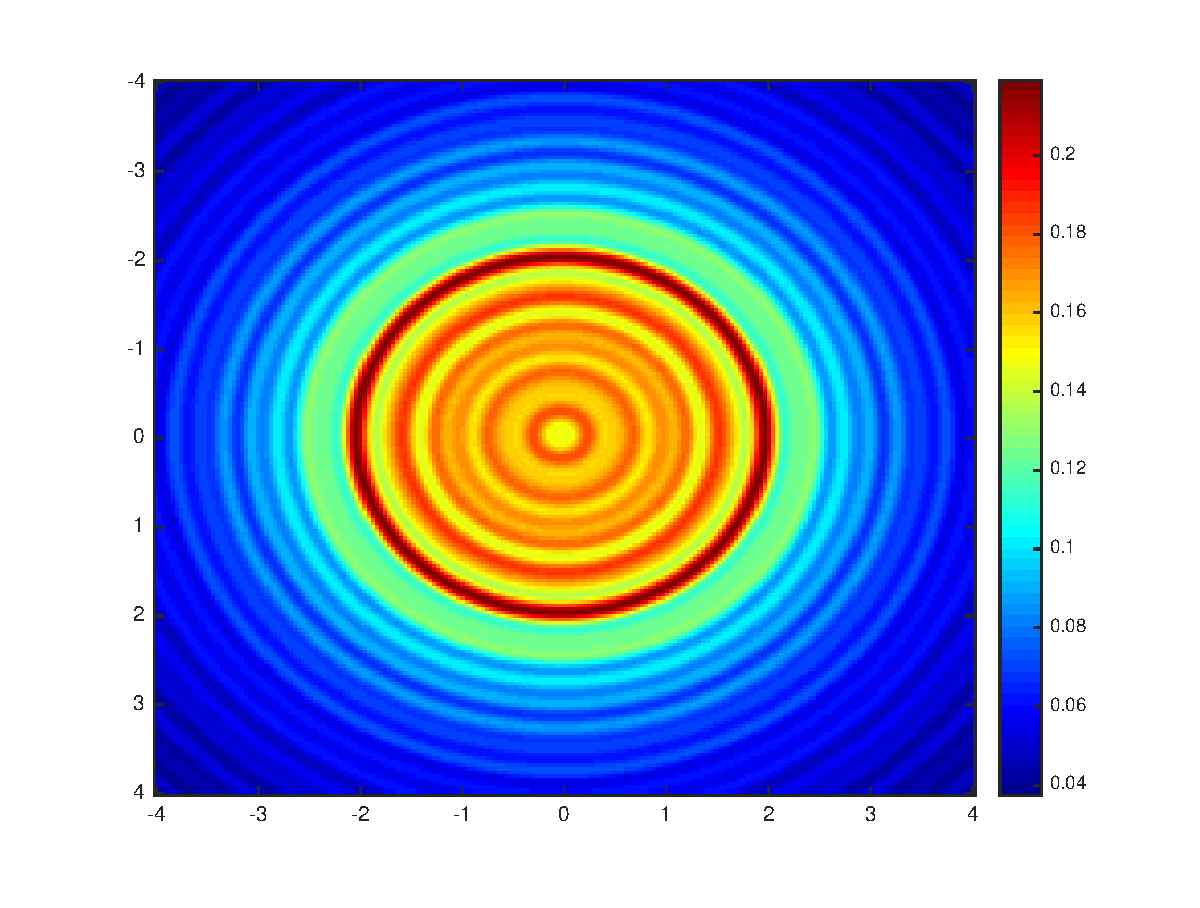
\includegraphics[width=0.24\textwidth]{./graphic_phase/circle_r_100_k_4_scalar.eps}
	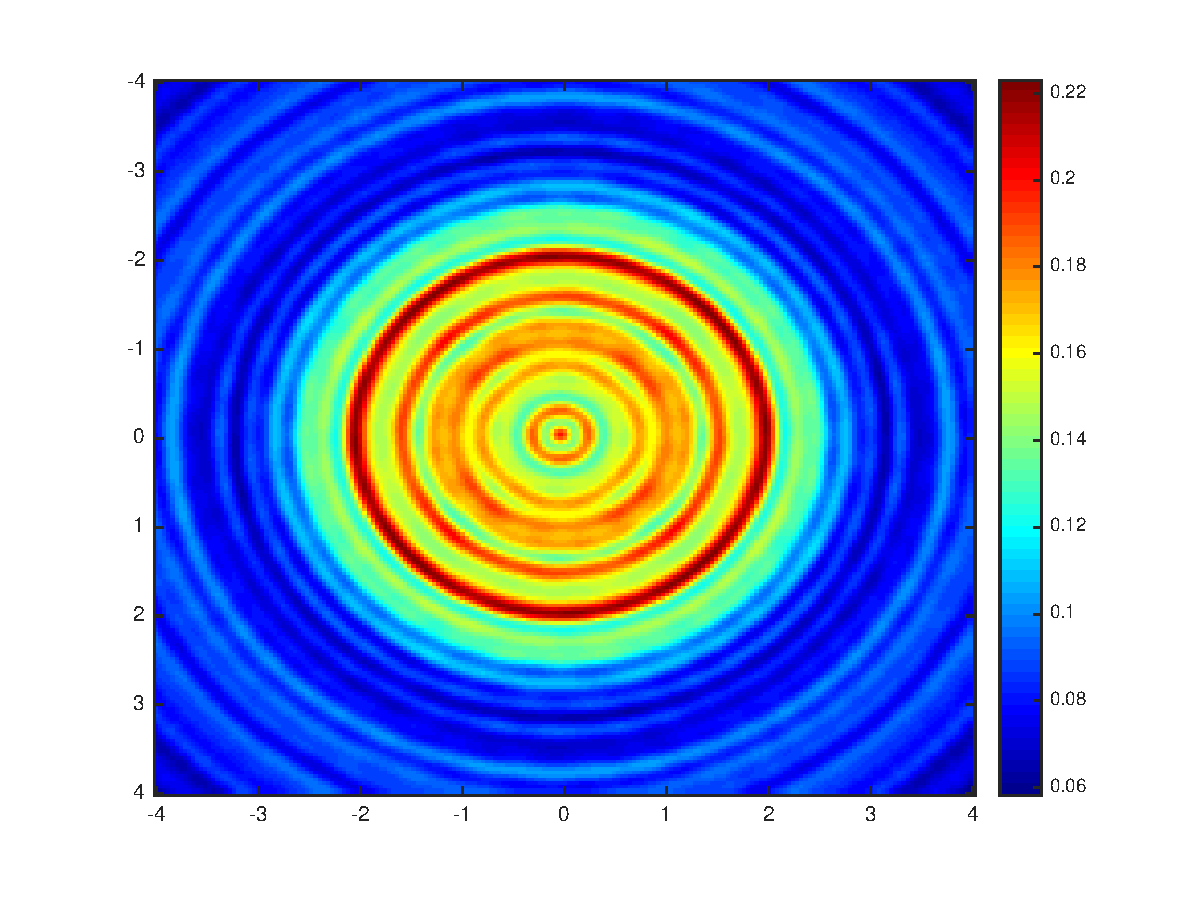
\includegraphics[width=0.24\textwidth]{./graphic_phase/circle_r_100_k_4_phaseless_n_128_bias_100.eps}
	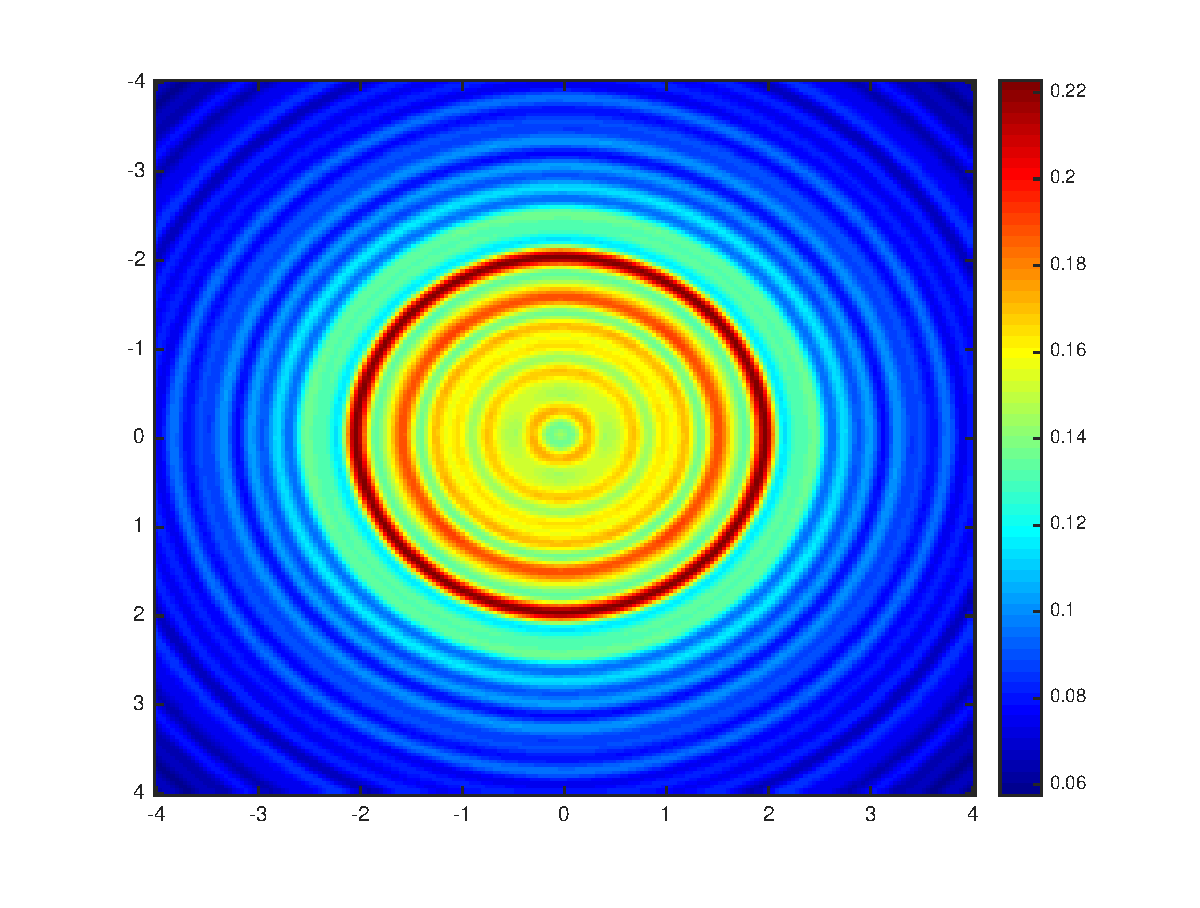
\includegraphics[width=0.24\textwidth]{./graphic_phase/circle_r_100_k_4_phaseless_n_512_bias_100.eps}
	
	\caption{Circle;From left to right: vector imaging, scalar imaging, phaseless imaging128, phaseless imaging512; From up to down: R=10, R=100 }\label{figure_circle_phaless}
\end{figure}
\begin{figure}
	\centering
	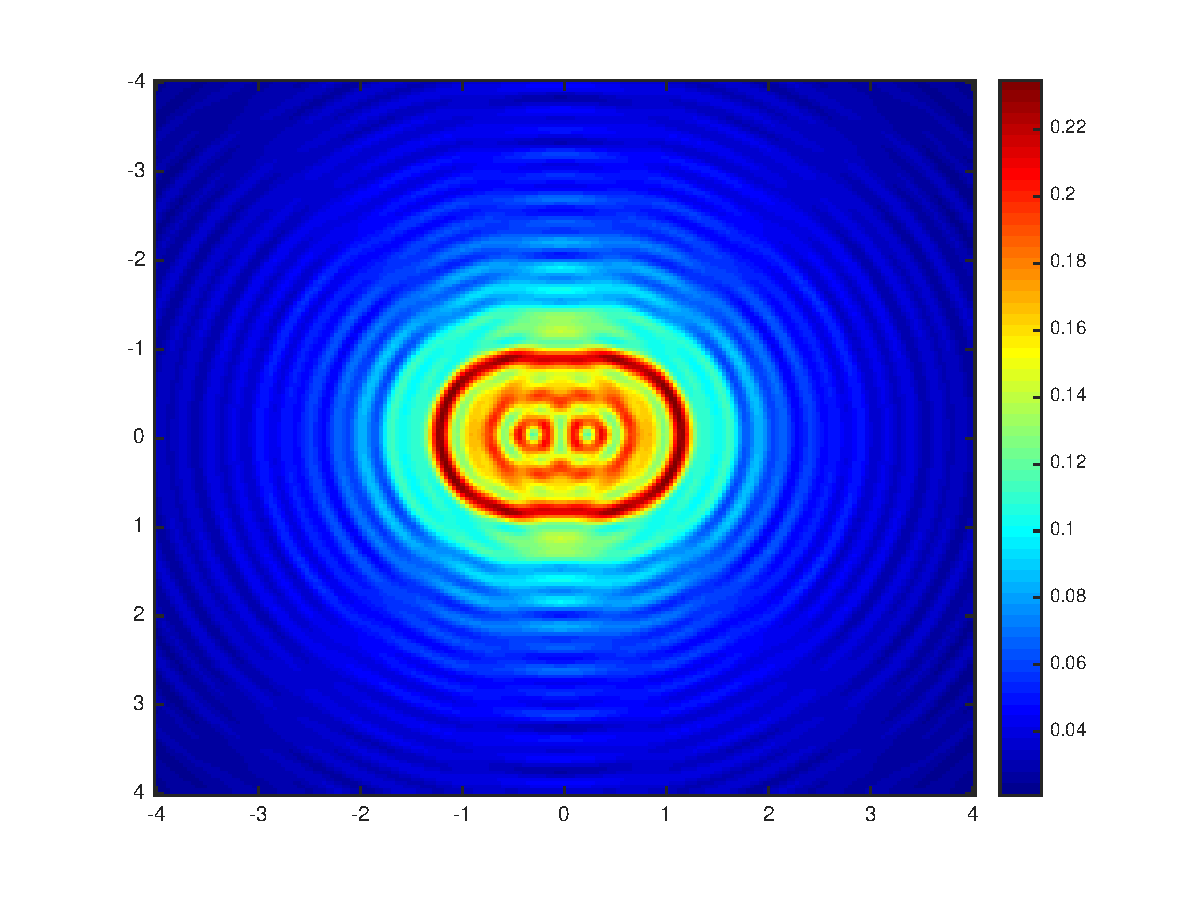
\includegraphics[width=0.24\textwidth]{./graphic_phase/peanut_r_10_k_4_vector.eps}
	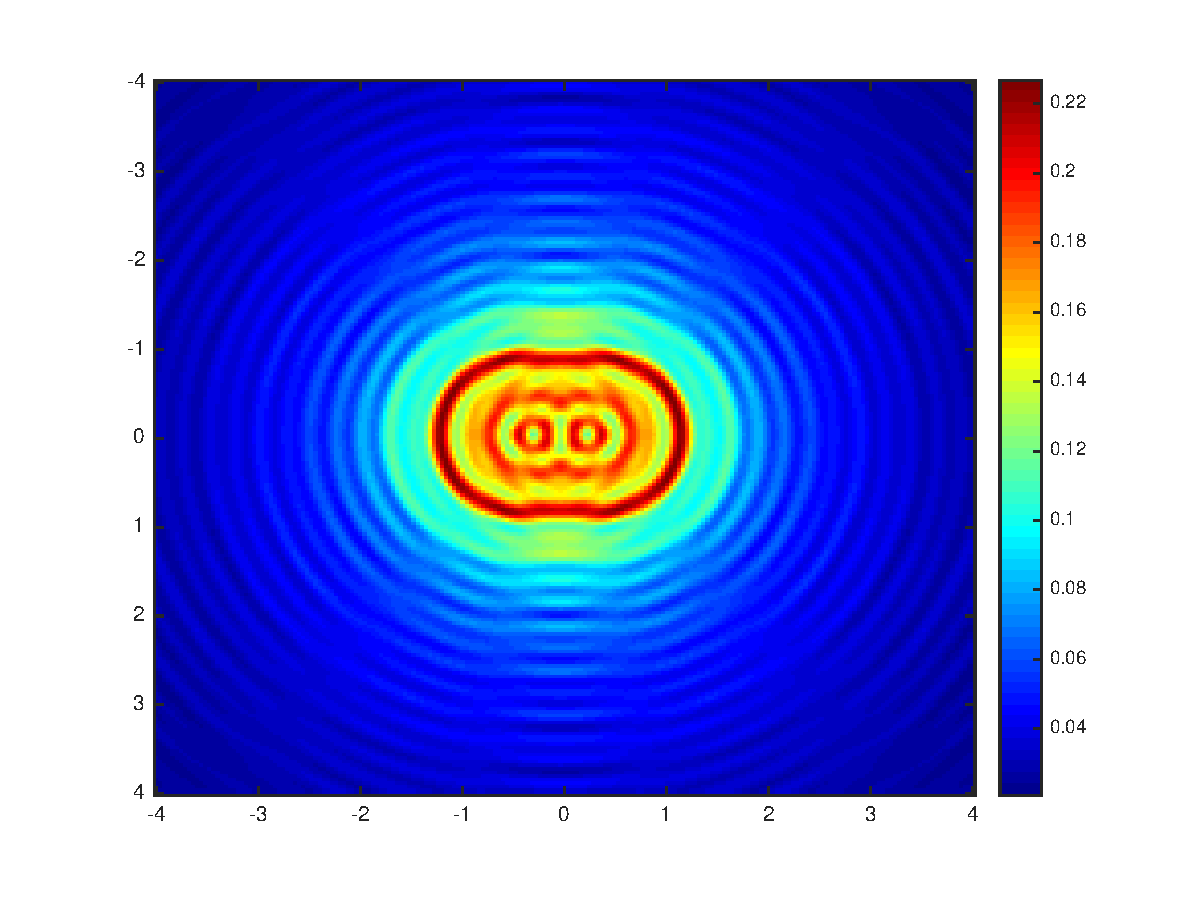
\includegraphics[width=0.24\textwidth]{./graphic_phase/peanut_r_10_k_4_scalar.eps}
	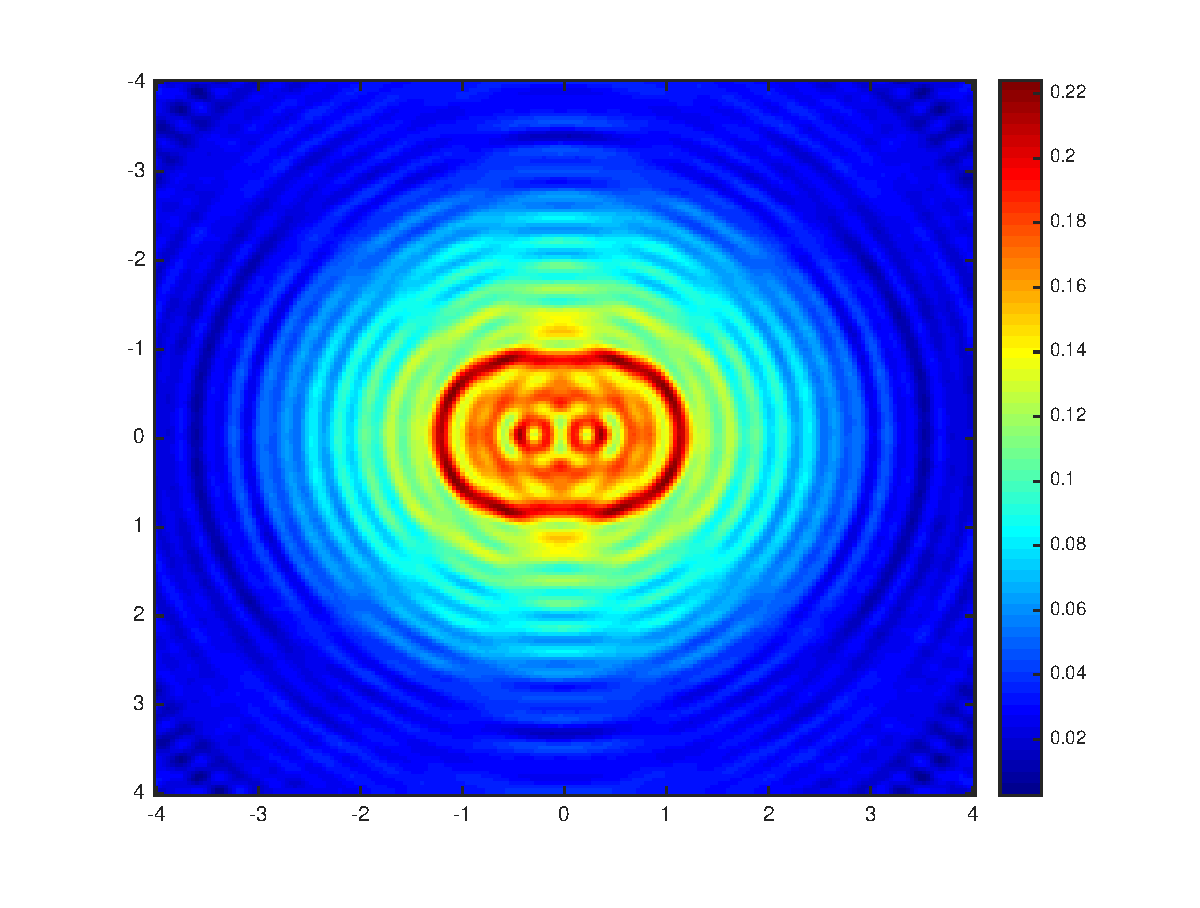
\includegraphics[width=0.24\textwidth]{./graphic_phase/peanut_r_10_k_4_phaseless_n_128_bias_100.eps}
	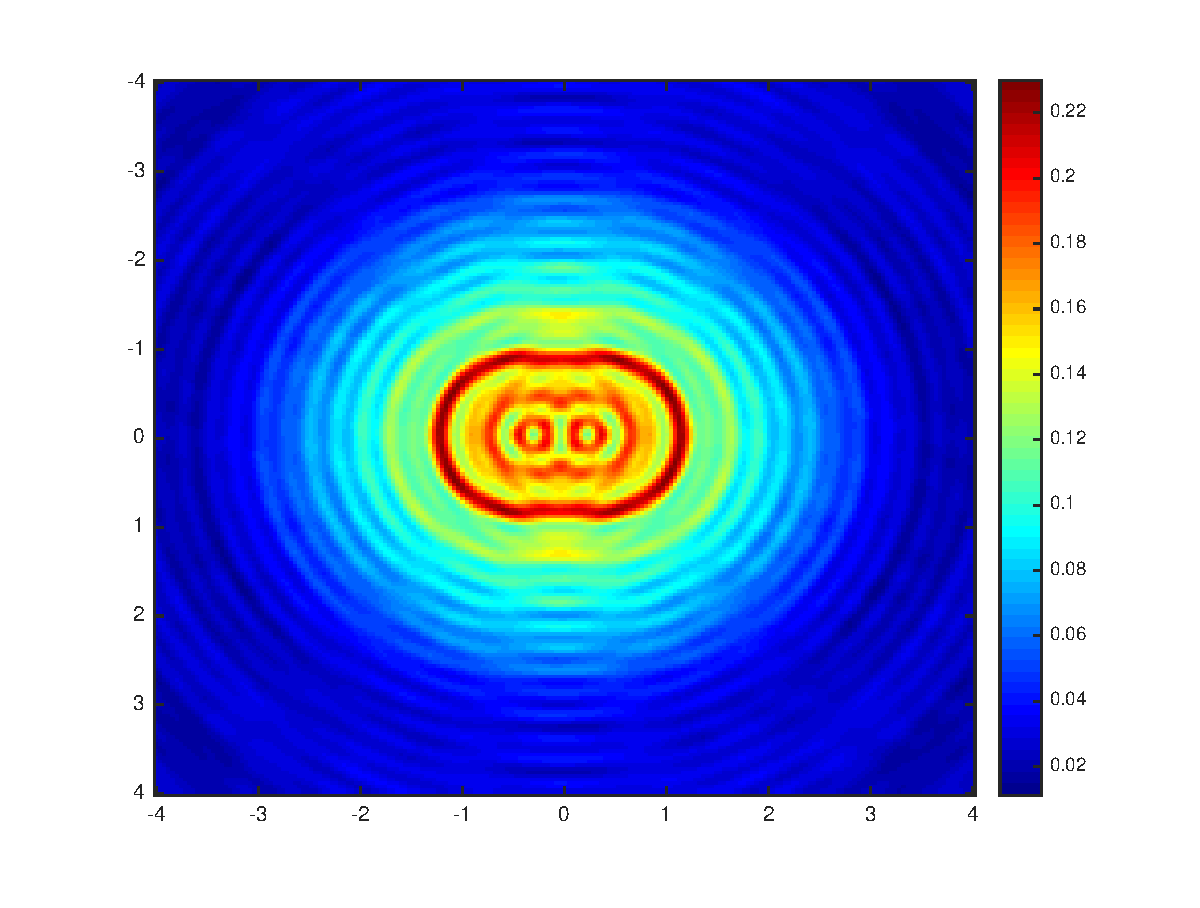
\includegraphics[width=0.24\textwidth]{./graphic_phase/peanut_r_10_k_4_phaseless_n_512_bias_100.eps}
	\caption{Peanut;From left to right: vector imaging, scalar imaging, phaseless imaging128, phaseless imaging512;  }\label{figure_peanut_phaless}
\end{figure}
\begin{figure}
	\centering
	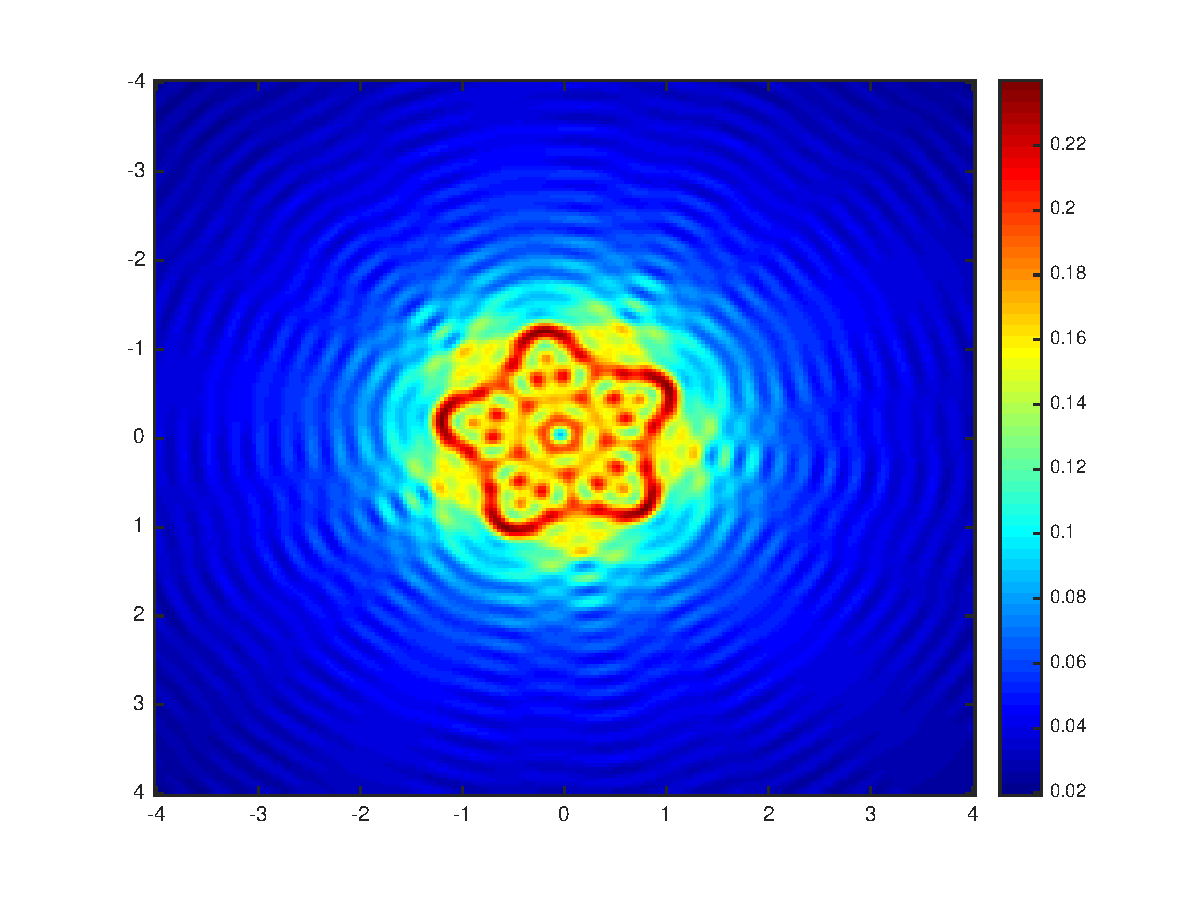
\includegraphics[width=0.24\textwidth]{./graphic_phase/5-leaf_r_10_k_4_vector.eps}
	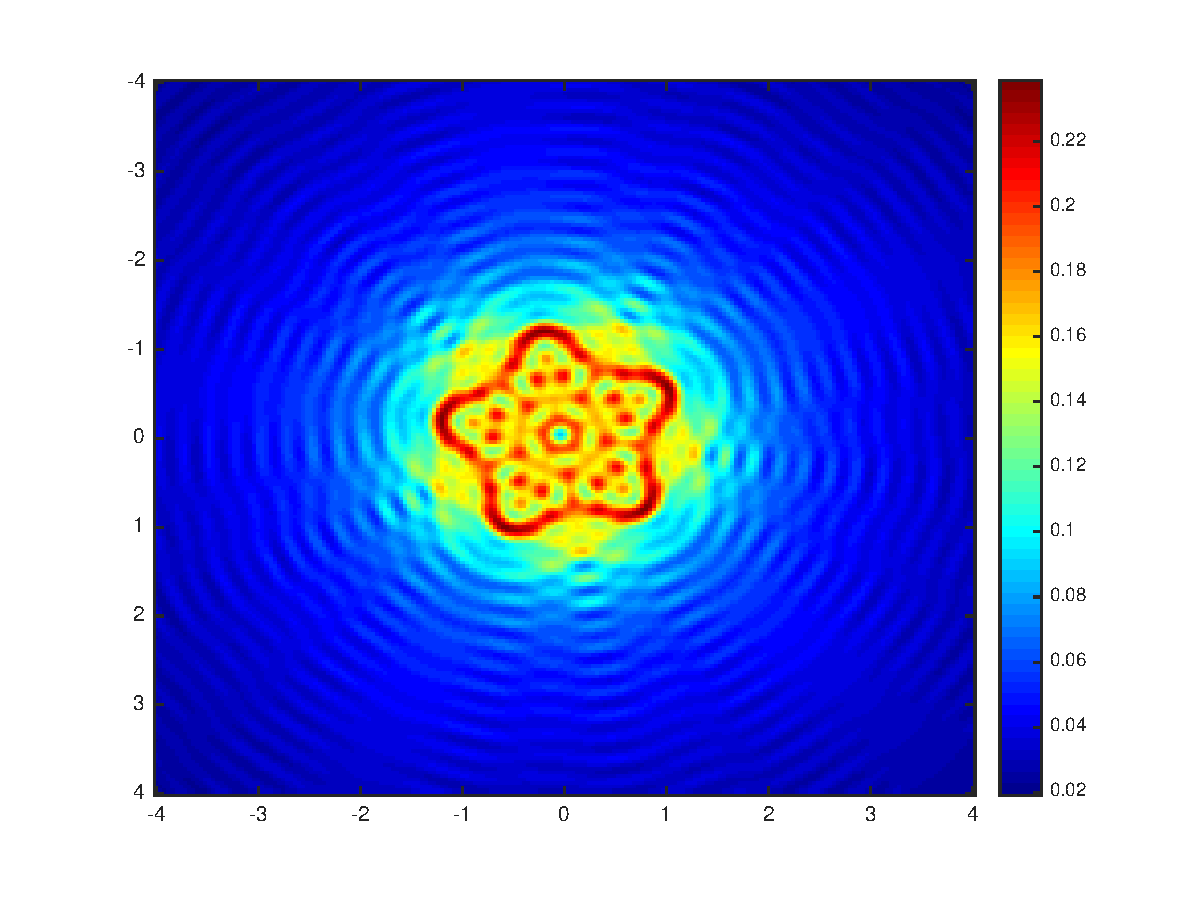
\includegraphics[width=0.24\textwidth]{./graphic_phase/5-leaf_r_10_k_4_scalar.eps}
	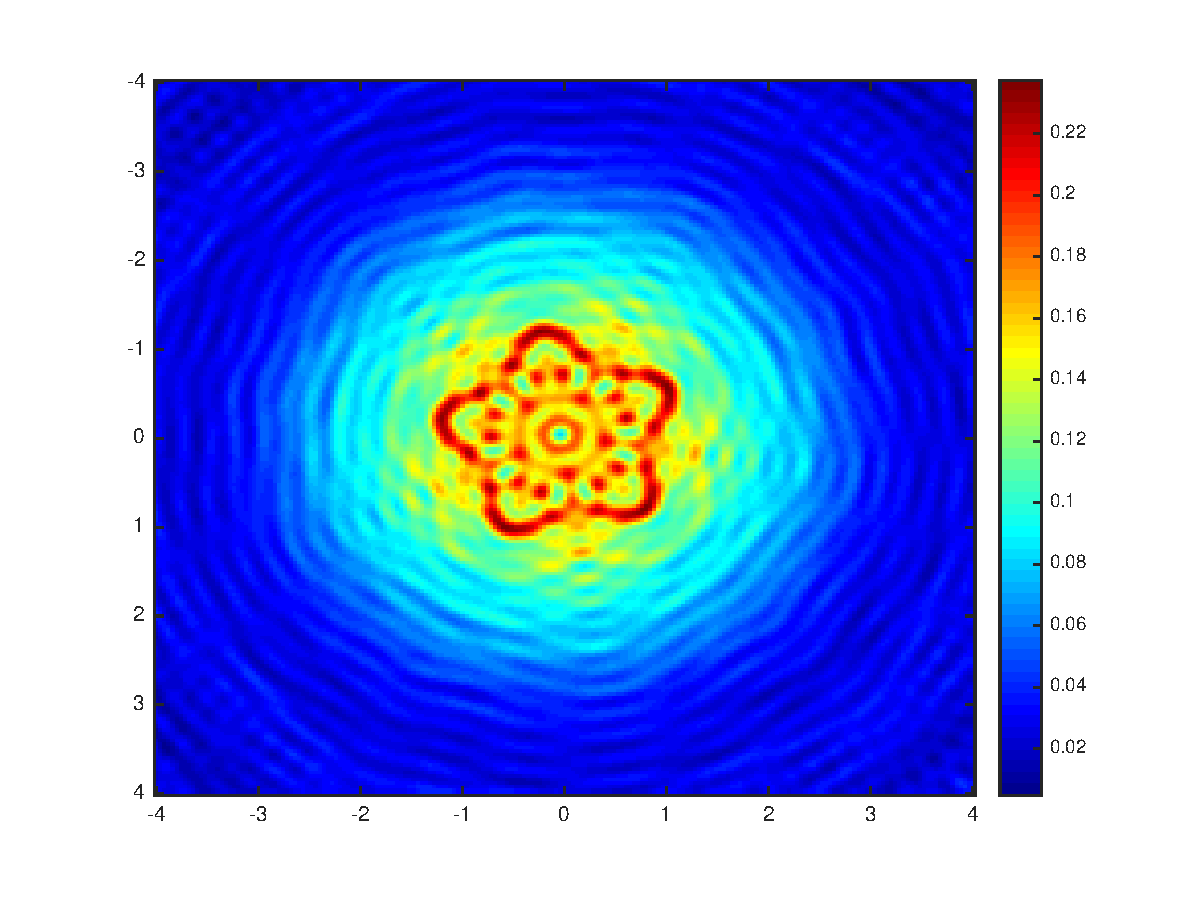
\includegraphics[width=0.24\textwidth]{./graphic_phase/5-leaf_r_10_k_4_phaseless_n_128_bias_100.eps}
	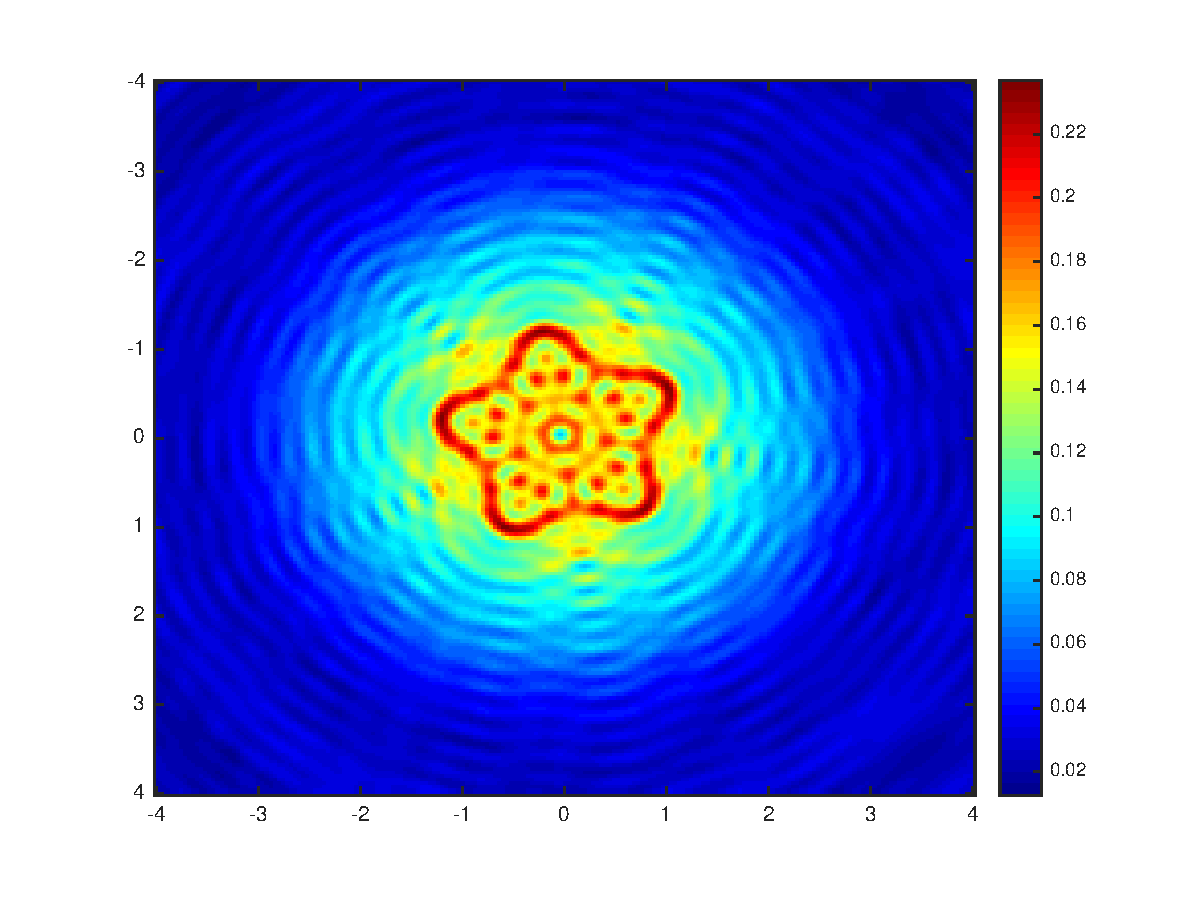
\includegraphics[width=0.24\textwidth]{./graphic_phase/5-leaf_r_10_k_4_phaseless_n_512_bias_100.eps}
	\caption{Peanut;From left to right: vector imaging, scalar imaging, phaseless imaging128, phaseless imaging512;  }\label{figure_5-leaf_phaless}
\end{figure}

\begin{figure}
	\centering
	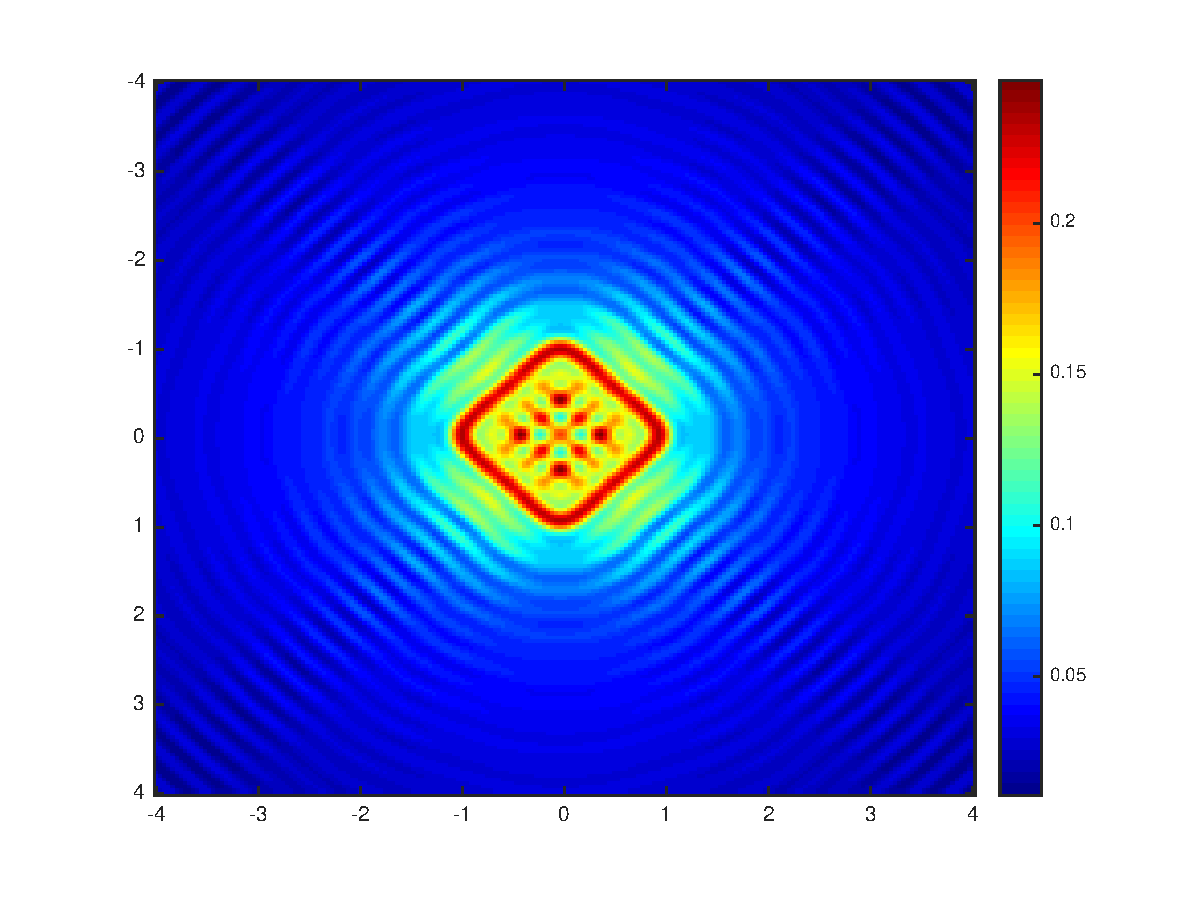
\includegraphics[width=0.24\textwidth]{./graphic_phase/rectangle_r_10_k_4_vector.eps}
	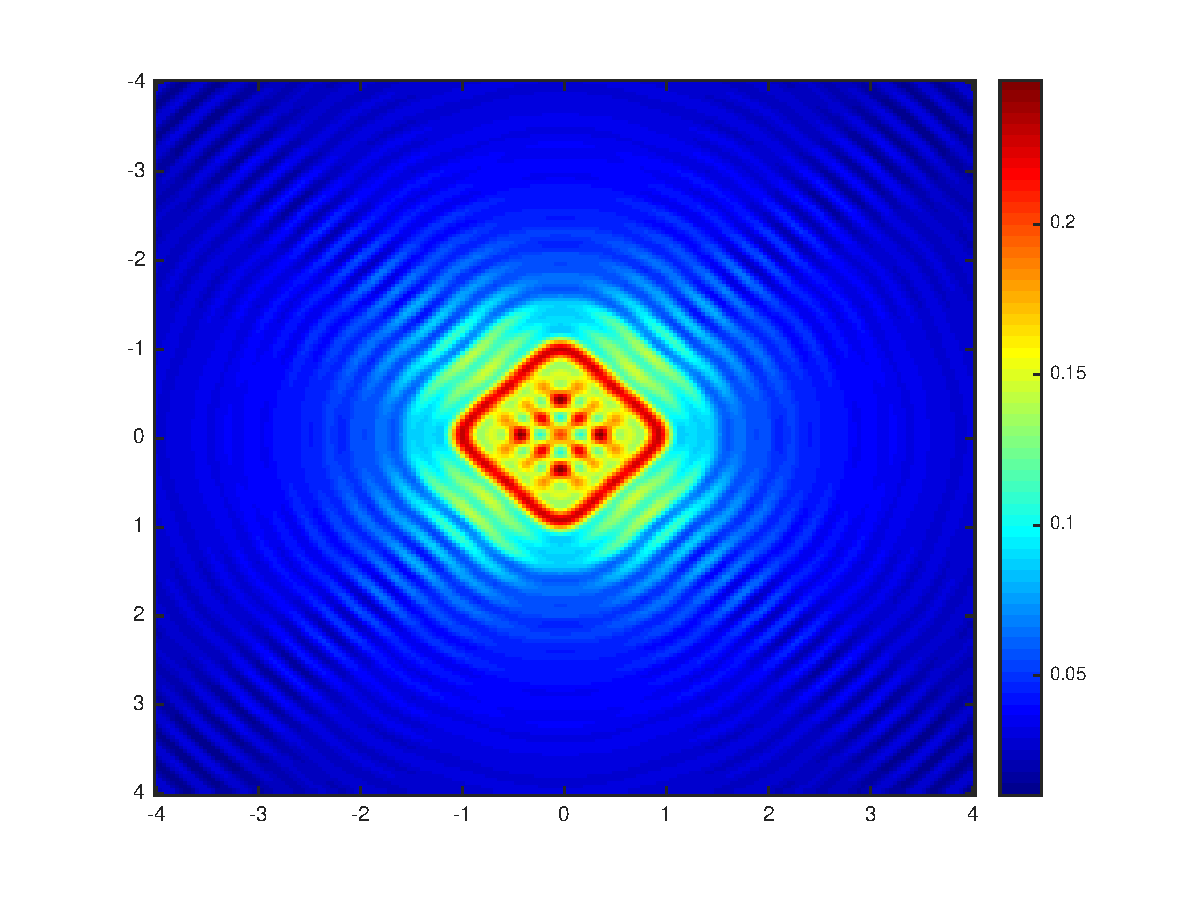
\includegraphics[width=0.24\textwidth]{./graphic_phase/rectangle_r_10_k_4_scalar.eps}
	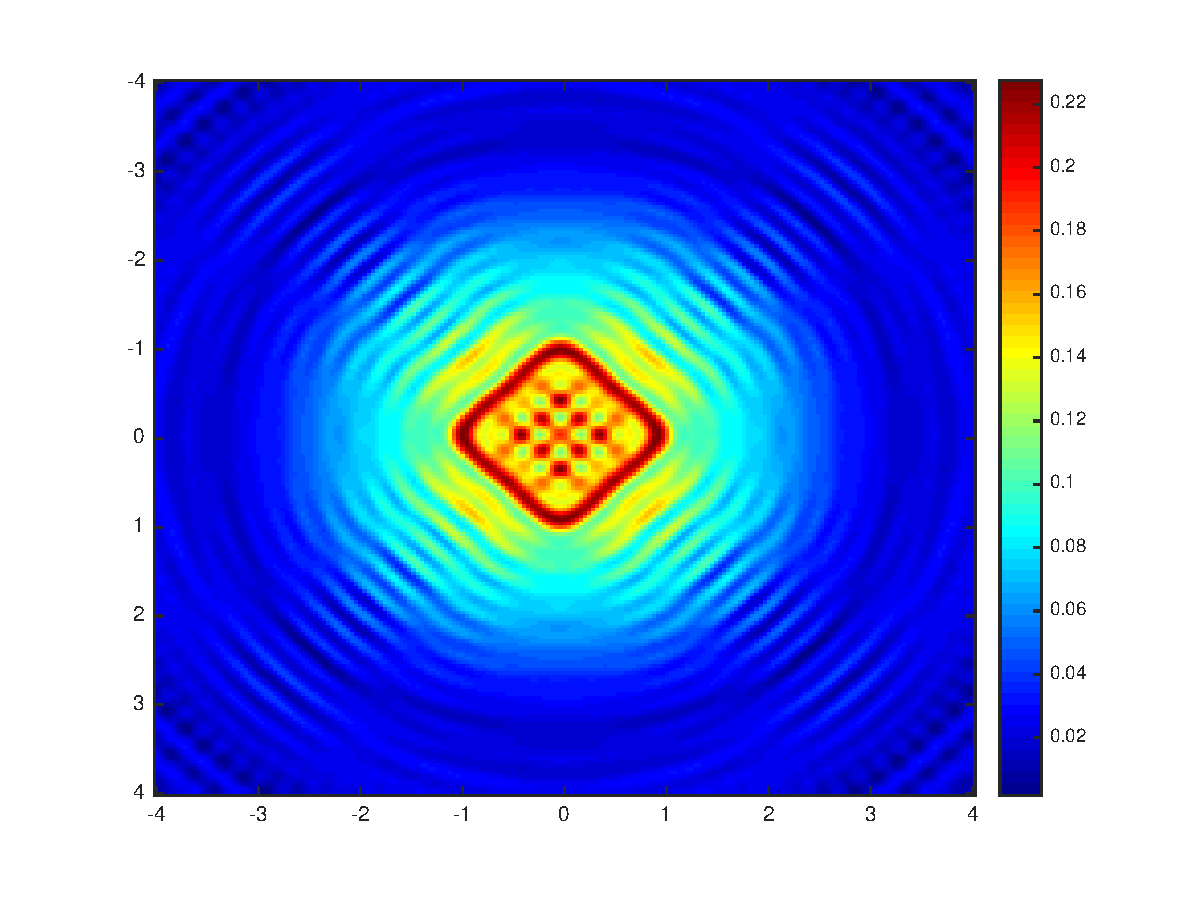
\includegraphics[width=0.24\textwidth]{./graphic_phase/rectangle_r_10_k_4_phaseless_n_128_bias_100.eps}
	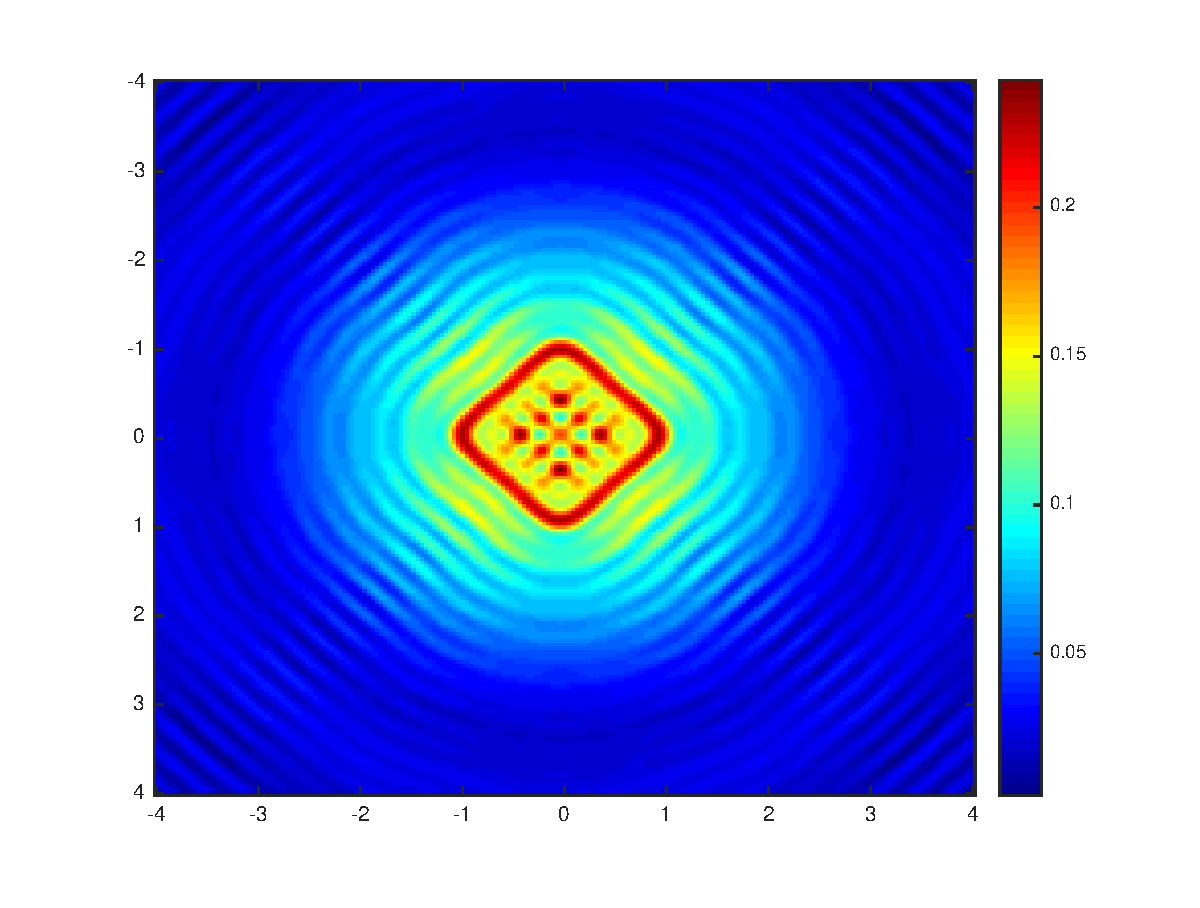
\includegraphics[width=0.24\textwidth]{./graphic_phase/rectangle_r_10_k_4_phaseless_n_512_bias_100.eps}
	\caption{Peanut;From left to right: vector imaging, scalar imaging, phaseless imaging128, phaseless imaging512;  }\label{figure_rectangle_phaless}
\end{figure}

\begin{figure}
	\centering
	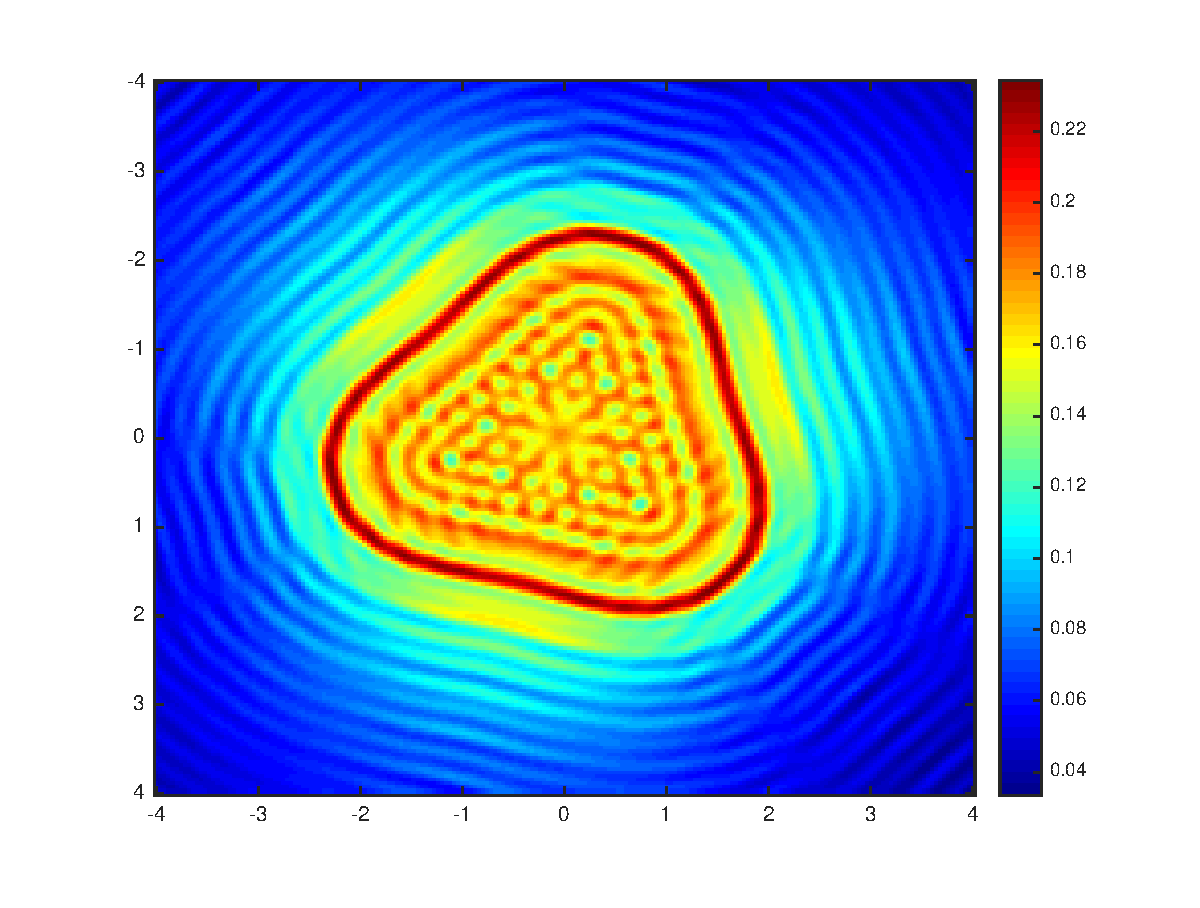
\includegraphics[width=0.24\textwidth]{./graphic_phase/pear_r_10_k_4_vector.eps}
	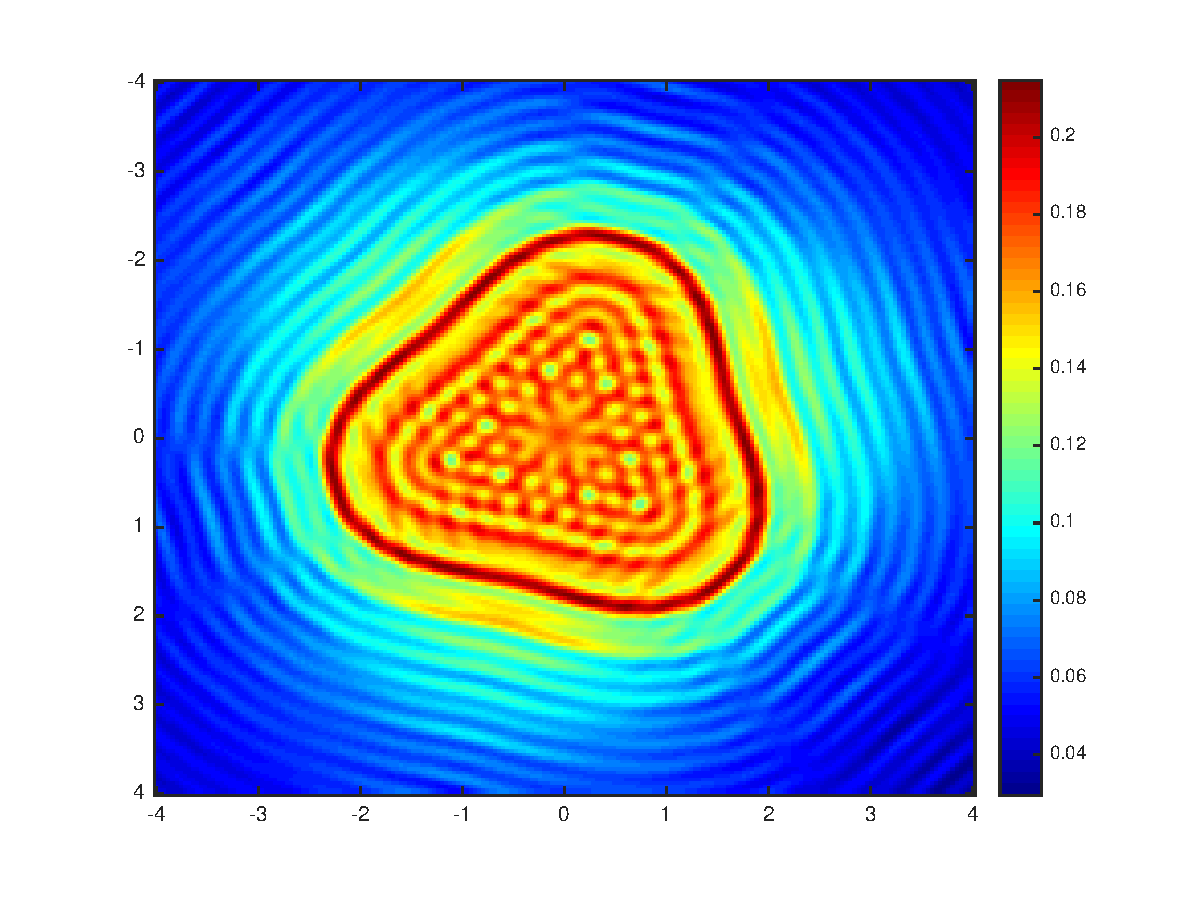
\includegraphics[width=0.24\textwidth]{./graphic_phase/pear_r_10_k_4_scalar.eps}
	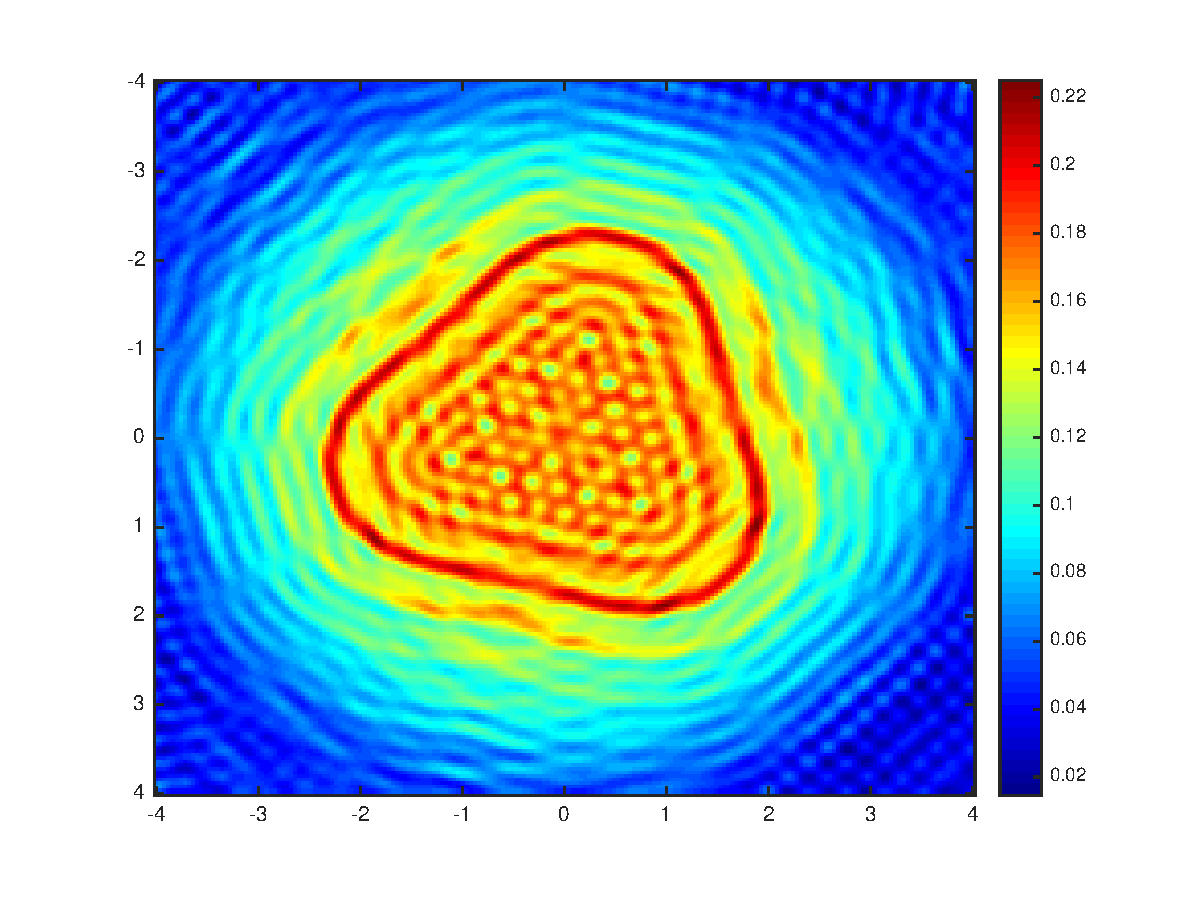
\includegraphics[width=0.24\textwidth]{./graphic_phase/pear_r_10_k_4_phaseless_n_128_bias_100.eps}
	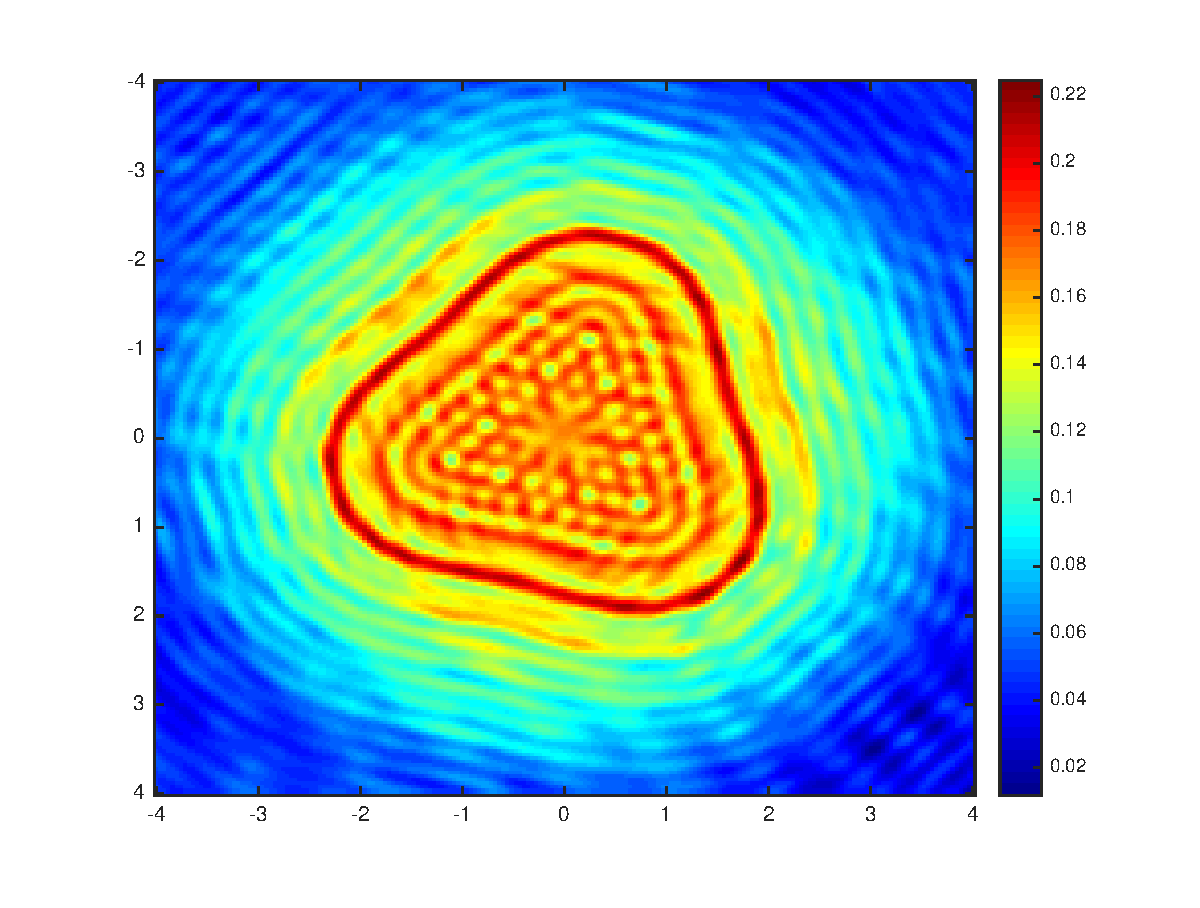
\includegraphics[width=0.24\textwidth]{./graphic_phase/pear_r_10_k_4_phaseless_n_512_bias_100.eps}
	\caption{Peanut;From left to right: vector imaging, scalar imaging, phaseless imaging128, phaseless imaging512;  }\label{figure_pear_phaless}
\end{figure}

\begin{figure}
	\centering
	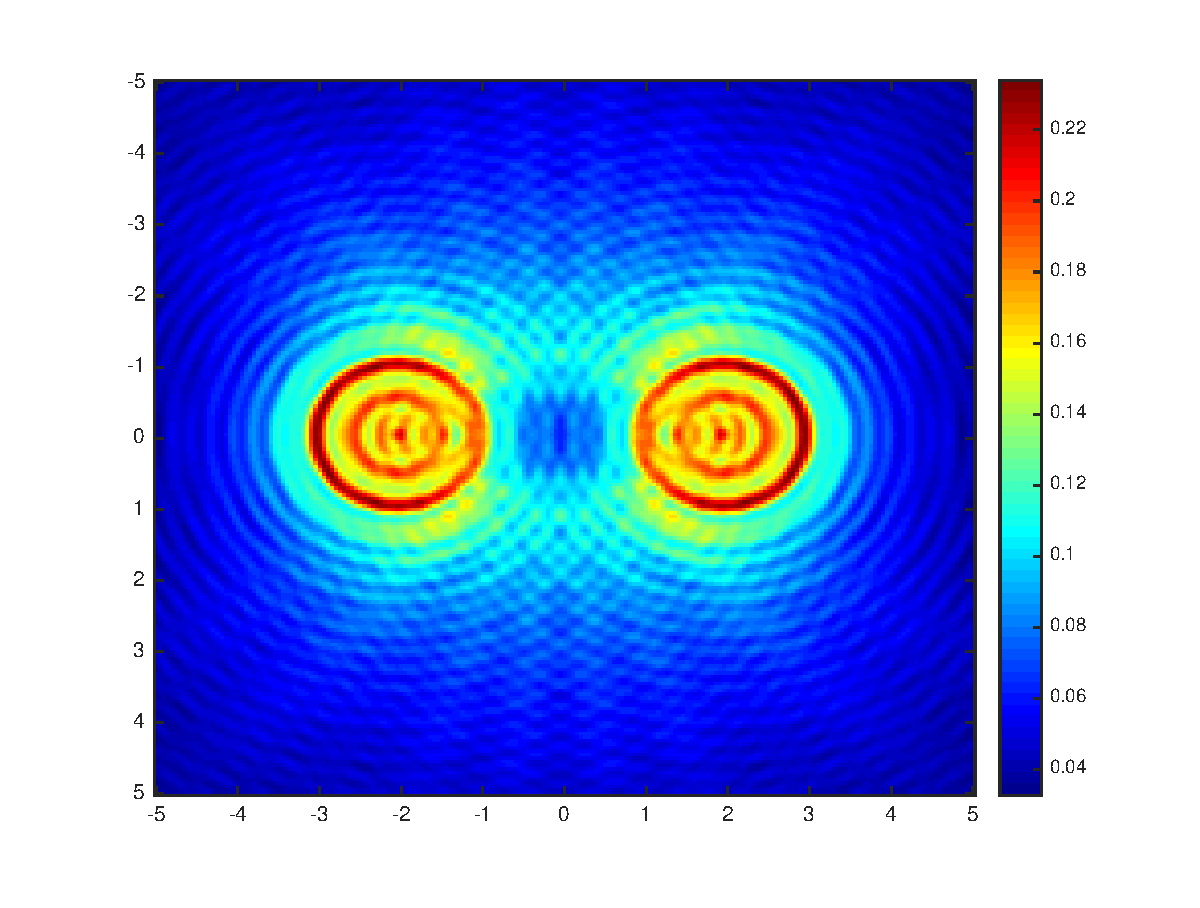
\includegraphics[width=0.24\textwidth]{./graphic_phase/bi_circle_r_10_k_4_vector.eps}
	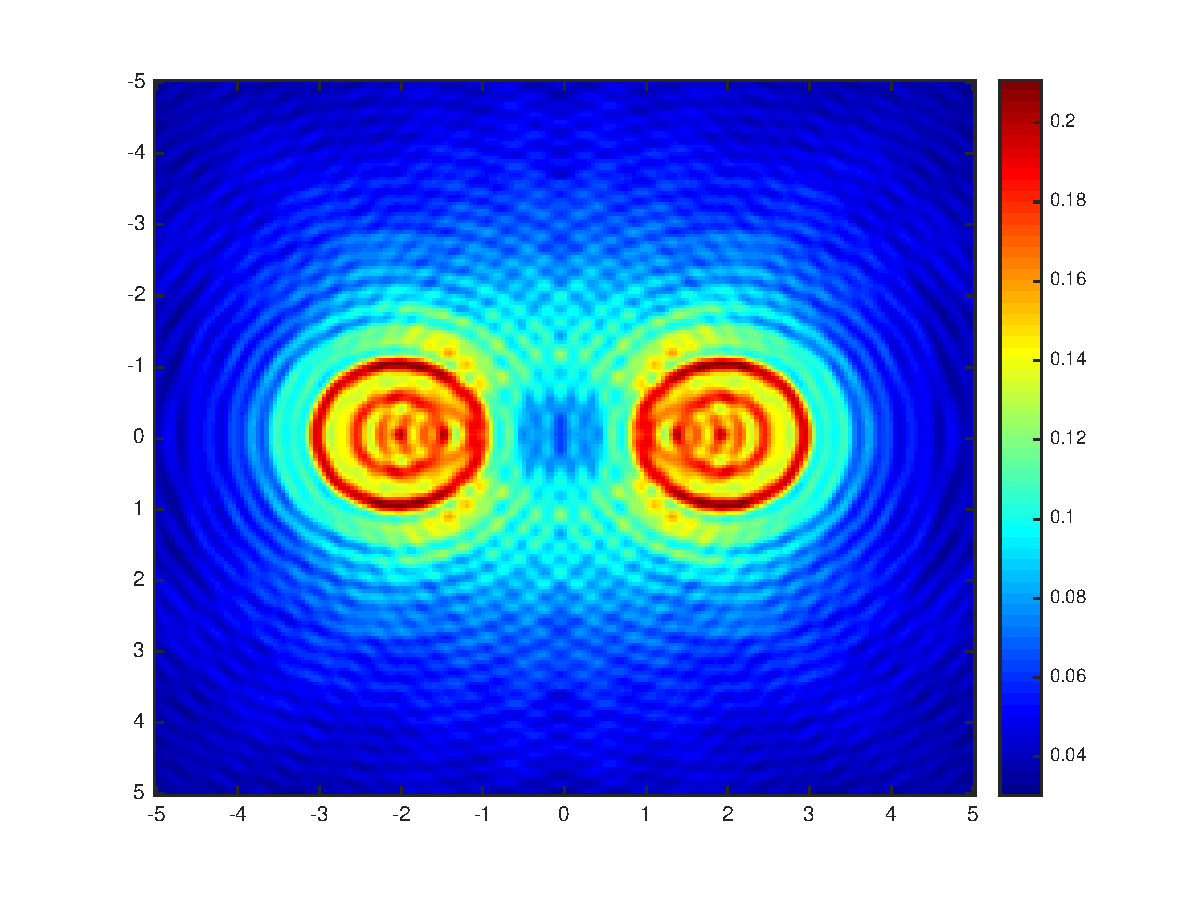
\includegraphics[width=0.24\textwidth]{./graphic_phase/bi_circle_r_10_k_4_scalar.eps}
	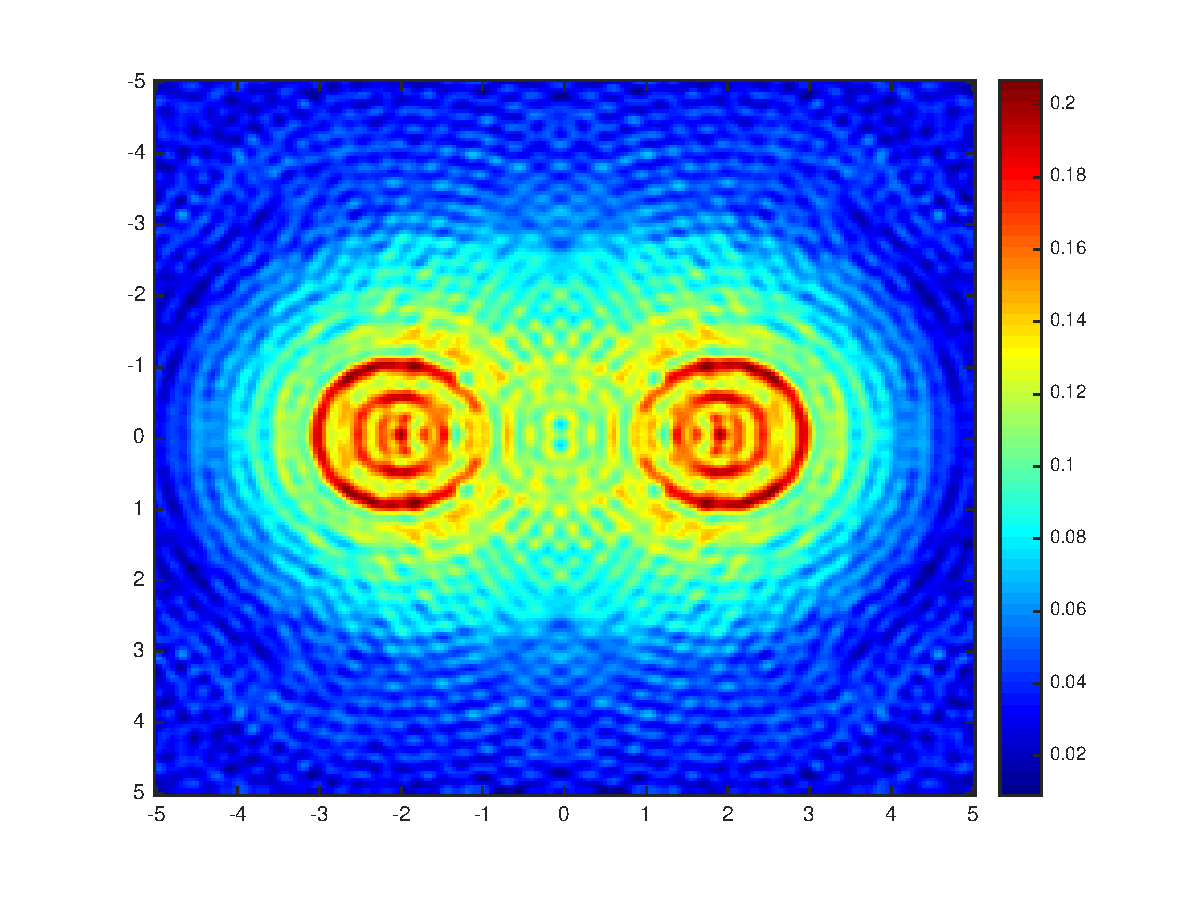
\includegraphics[width=0.24\textwidth]{./graphic_phase/bi_circle_r_10_k_4_phaseless_n_128_bias_100.eps}
	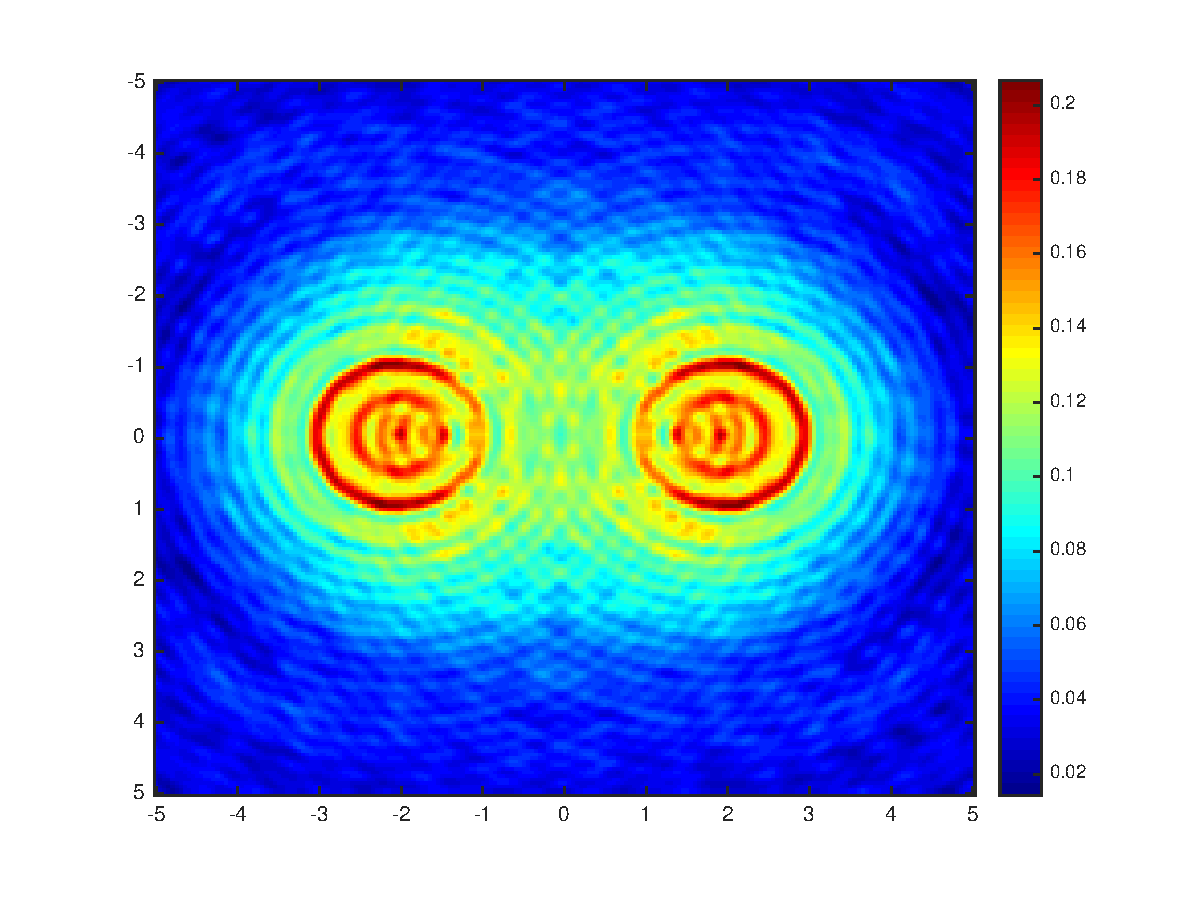
\includegraphics[width=0.24\textwidth]{./graphic_phase/bi_circle_r_10_k_4_phaseless_n_512_bias_100.eps}
	
	\caption{Circle;From left to right: vector imaging, scalar imaging, phaseless imaging128, phaseless imaging512; From up to down: R=10, R=100 }\label{figure_bicircle_phaless}
\end{figure}

\section*{References}
\bibliography{eee}
\end{document}
